\documentclass[a4paper]{article}

\usepackage[utf8]{inputenc}
\PassOptionsToPackage{hyphens}{url} % zodat url's ook afgekapt worden
\usepackage{hyperref}
\usepackage[dutch]{babel}
\usepackage{graphicx}
\graphicspath{{img/}}
\usepackage{algorithm}
\usepackage{algorithmic}
\usepackage[toc,page]{appendix}
\usepackage{mathtools}
\usepackage{tocbibind}
\usepackage{float}
\usepackage{framed}
\usepackage{parskip}
\usepackage{listings}
\usepackage{color}
\usepackage{pdfpages}
\usepackage{pdflscape}
\usepackage{todonotes}
\usepackage{tabularx}
\usepackage{usecases}
\usepackage{enumitem}

\begin{document}
%%%%%%%%%%%%%%%%%%%%%%%%%%%%%%%%%%%%%%%%%
% University Assignment Title Page 
% LaTeX Template
% Version 1.0 (27/12/12)
%
% This template has been downloaded from:
% http://www.LaTeXTemplates.com
%
% Original author:
% WikiBooks (http://en.wikibooks.org/wiki/LaTeX/Title_Creation)
%
% License:
% CC BY-NC-SA 3.0 (http://creativecommons.org/licenses/by-nc-sa/3.0/)
% 
% Instructions for using this template:
% This title page is capable of being compiled as is. This is not useful for 
% including it in another document. To do this, you have two options: 
%
% 1) Copy/paste everything between \begin{document} and \end{document} 
% starting at \begin{titlepage} and paste this into another LaTeX file where you 
% want your title page.
% OR
% 2) Remove everything outside the \begin{titlepage} and \end{titlepage} and 
% move this file to the same directory as the LaTeX file you wish to add it to. 
% Then add \input{./title_page_1.tex} to your LaTeX file where you want your
% title page.
%
%%%%%%%%%%%%%%%%%%%%%%%%%%%%%%%%%%%%%%%%%

%----------------------------------------------------------------------------------------
%	PACKAGES AND OTHER DOCUMENT CONFIGURATIONS
%----------------------------------------------------------------------------------------
\begin{titlepage}
\pagestyle{empty}
\newcommand{\HRule}{\rule{\linewidth}{0.5mm}} % Defines a new command for the horizontal lines, change thickness here

\center % Center everything on the page
 
%----------------------------------------------------------------------------------------
%	HEADING SECTIONS
%----------------------------------------------------------------------------------------

\textsc{\LARGE Universiteit Hasselt}\\[1.5cm] % Name of your university/college
\textsc{\Large Software Engineering}\\[0.5cm] % Major heading such as course name
\textsc{\large Requirements analyse }\\[0.5cm] % Minor heading such as course title
% \textsc{\LARGE Modulo}\\[0.5cm] % Minor heading such as course title

%----------------------------------------------------------------------------------------
%	TITLE SECTION
%----------------------------------------------------------------------------------------

\HRule \\[0.4cm]
%{ \huge \bfseries Managementsysteem \\ Deeltijds Onderwijs }\\[0.2cm] % Title of your document
{ \huge \bfseries Modulo \\ \vspace{-0.4em} ----- \vspace{-0.4em}\\ Managementsysteem \\ Deeltijds Onderwijs }\\[0.2cm] % Title of your document
\HRule \\[1.5cm]
 
%----------------------------------------------------------------------------------------
%	AUTHOR SECTION
%----------------------------------------------------------------------------------------

\begin{minipage}{0.4\textwidth}
\begin{flushleft} \large
\emph{Auteurs:}\\
Vincent \textsc{Drozdzyniak} % Your name
Hendrik \textsc{Lievens} \\ 
Martijn \textsc{Maes} \\
Reinaert \textsc{Van de Cruys} \\
Michiel \textsc{Vanmunster} \\
Jens \textsc{Vannitsen}
\end{flushleft}
\end{minipage}
~
\begin{minipage}{0.4\textwidth}
\begin{flushright} \large
% \emph{Promotor:} \\
% Prof. dr. Frank \textsc{Neven}\\ % Supervisor's Name
% \vspace{4mm}
\emph{Begeleider:} \\
Robin \textsc{Marx}
\end{flushright}
\end{minipage}\\[2.5cm]

% If you don't want a supervisor, uncomment the two lines below and remove the section above
%\Large \emph{Author:}\\
%John \textsc{Smith}\\[3cm] % Your name


%----------------------------------------------------------------------------------------
%	DATE SECTION
%----------------------------------------------------------------------------------------

{\large 17 maart 2016}\\[2cm] % Date, change the \today to a set date if you want to be precise

%----------------------------------------------------------------------------------------
%	LOGO SECTION
%----------------------------------------------------------------------------------------


\includegraphics[width=0.4\textwidth]{UH_logo}\\[2cm] % Include a department/university logo - this will require the graphicx package
 
%----------------------------------------------------------------------------------------

\vfill % Fill the rest of the page with whitespace

\end{titlepage}

\tableofcontents
\newpage

\section{Preface}
Dit document is bedoeld voor het personeel van het Technisch Instituut Heilig Hart te Hasselt \cite{TIHH} zijnde de opdrachtgevers, voor het onderwijsteam en het ontwikkelingsteam van Modulo. In dit document worden alle vereisten van het softwarepakket geanalyseerd.


\section{Inleiding}
Modulo is een Managementsysteem voor het Deeltijds Onderwijs (MDO) dat gebruikt kan worden in alle onderwijsinstellingen waar het Deeltijds Beroepssecundair Onderwijs (DBSO) \cite{DBSO} als onderwijsvorm wordt gehanteerd. Dit omvat alle Centra voor Deeltijds Onderwijs (CDO) \cite{CDO} alsook het Syntra-netwerk \cite{Syntra}.

%DBSO is een onderwijsvorm waarin studenten leren op school combineren met leren op werkplekken. Een opleiding duurt drie jaar, bestaande uit de vakken BGV en PAV. Een lesweek bestaat uit 8 uur BGV en 7 uur PAV. De rest van de tijd brengen de studenten door op de werkvloer, wat ook tot BGV gerekend wordt. Tijdens het vak PAV moeten de studenten voor iedere graad doelstellingen verwerven die opgelegd zijn door de overheid (leerplan). Wanneer men voor alle graden, alle doelstelling verworven heeft, krijgt de student het diploma secundair onderwijs. Tijdens de BGV vakken leert men een beroep aan. Om een beroep uit te kunnen oefenen heb je het certificaat nodig van dat beroep. Dit certificaat kan je verkrijgen tijdens de BGV lessen. Iedere certificaat is opgedeeld in deelcertificaten en ieder van deze deelcertificaten bestaat uit competenties. Je verkrijgt een certificaat wanneer je alle deelcertificaten verworven hebt. Een deelcertificaat verkrijg je als je alle competenties van dit certificaat verworven hebt. Met de invoering van het duaal leren \cite{Duaal_leren} zal Modulo ook in alle beroeps- en technische richtingen gebruikt kunnen worden. 

In sectie \ref{sec:general_descr} wordt allereerst een algemeen beeld gegeven van de werking van het DBSO en de precieze rol die Modulo daarin kan spelen. Vervolgens worden in sectie \ref{sec:user_req} alle vereisten van het softwarepakket tegenover de gebruiker besproken. Er wordt een uitgebreide lijst van vereiste functionaliteiten gegeven, alsook een analyse van het gebruik, de mogelijkheden voor ondersteuning en de juridische aspecten. Sectie \ref{sec:systeemarchitectuur} biedt een uiteenzetting van de gekozen technologieën om het softwarepakket te implementeren en in sectie \ref{sec:use_cases} wordt dieper ingegaan op de concrete stappen die verschillende types gebruikers moeten doorlopen om bepaalde acties te ondernemen. In de appendices tenslotte kunnen mockups gevonden worden die tonen hoe Modulo er voor de gebruiker uitziet.

\section{Woordenlijst}  \label{sec:word_list} % voor de klant
\def\arraystretch{1.8}
\begin{tabularx}{\textwidth}{l | X}
    Term & Definitie \\
    \hline \hline
    MDO &`Managementsysteem voor het Deeltijds Onderwijs' is het antwoord op de vraag ``Wat is Modulo?''. Het is een softwarepakket voor het beheren van de gegevens van studenten binnen het DBSO. \\
    \hline
    DBSO & `Deeltijds Beroepssecundair Onderwijs', of kortweg `deeltijds onderwijs', is een onderwijsvorm waarin studenten `leren op school' combineren met `leren op werkplekken'. Een lesweek bestaat uit 8 uur `Beroepsgerichte Vorming' (BGV) en 7 uur `Project Algemene Vakken' (PAV), de rest van de tijd brengen de studenten door op de werkvloer. \cite{DBSO} \\
    \hline
    CDO & `Centra voor Deeltijds Onderwijs' zijn scholen die DBSO als onderwijsvorm hanteren. De opdrachtgever voor Modulo, het Technisch Instituut Heilig Hart te Hasselt \cite{TIHH}, is hier een voorbeeld van. \cite{CDO} \\
\end{tabularx}

\newpage
\begin{tabularx}{\textwidth}{l | X}
    Term & Definitie \\
    \hline \hline
    BGV & `Beroepsgerichte Vorming' is het vak binnen het DBSO dat alle beroepsspecifieke competenties voor een opleiding omvat en zo de studenten alle kennis en vaardigheden bijbrengt die ze op de werkvloer nodig hebben. \\
    \hline
    PAV & `Project Algemene Vorming' of `Project Algemene Vakken' is het vak binnen het DBSO dat alle doelstellingen van de 2de en 3de graad omvat, zodat de studenten hun diploma secundair onderwijs kunnen behalen. \\
    \hline
    Competentie & Het certificaat dat door middel van BGV verkregen kan worden, bestaat uit een verzameling deelcertificaten. Ieder deelcertificaat bestaat uit een lijst van competenties, vastgelegd door de Vlaamse overheid, die de studenten allemaal moeten halen om het deelcertificaat te verkrijgen. Een deelcertificaat kan op andere deelcertificaten voortbouwen, die dan ook in volgorde behaald moeten worden. \cite{Competenties} \\
    \hline
    Doelstelling & Doelstellingen zijn eindtermen voor het secundair onderwijs die per graad door de Vlaamse overheid zijn vastgelegd. Studenten moeten alle doelstellingen van alle graden behalen alvorens ze het diploma secundair onderwijs kunnen ontvangen. Binnen het DBSO zijn al deze doelstellingen ondergebracht in het vak PAV. De leerkrachten delen de doelstellingen op in samenhangende gehelen, zogeheten vakthema's, en brengen de doelstellingen vervolgens thema per thema bij aan de studenten. \cite{Doelstellingen} \\
    \hline
    A,I,V & A (aangeboden), I (ingeoefend) en V (verworven) zijn de drie mogelijke toestanden die een aangeboden competentie of doelstelling op een bepaalde dag toegewezen kan krijgen. Indien de leerkracht `verworven' invult, betekent dit dat de student heeft aangetoond de competentie of doelstelling te beheersen, `ingeoefend' betekent dat de student inzet heeft getoond om de competentie of doelstelling te behalen maar deze nog niet volledig onder de knie heeft, en `aangeboden' betekent dat de student zich niet heeft ingezet of afwezig was. Binnen het TIHH (Technisch Instituut Heilig Hart), de opdrachtgever van dit softwarepakket, wordt een competentie of doelstelling pas als behaald beschouwd wanneer de student er drie keer een V (verworven) voor heeft gescoord, op drie verschillende dagen. Daarna wordt de student niet meer op de betreffende competentie of doelstelling beoordeeld.
\end{tabularx}


\newpage
\section{Algemene beschrijving}  \label{sec:general_descr}% voor de klant
\subsection{Deeltijds beroepssecundair onderwijs}
Studenten in het secundair onderwijs kunnen vanaf de tweede graad overstappen op het DBSO. Hier kunnen ze een praktijkgerichte opleiding volgen die zorgt dat ze klaar zijn om een specifiek beroep van hun keuze uit te oefenen aan het einde van hun middelbare opleiding.

Het DBSO heeft slechts twee lesdagen waarop twee vakken worden aangeboden: BGV en PAV (zie sectie \ref{sec:word_list} voor meer uitleg over deze en volgende termen). De resterende drie weekdagen brengen de studenten door als jobstudent in een bedrijf.

Het doel van BGV is om de studenten alle kennis en vaardigheden bij te brengen die ze op de werkvloer nodig hebben. De inhoud van BGV hangt dan ook sterk af van de opleiding die de student volgt; BGV heeft een heel andere inhoud in de opleiding Metselaar dan in de opleiding Kok. Aan het einde van de opleiding krijgt de student een certificaat voor die opleiding uitgereikt. Om dit te behalen, moet de student eerst alle deelcertificaten binnen dit certificaat behalen (in het geval van Metselaar zijn dit er zes, waaronder `Basistechnieken metselwerk', `Bekisting' en `Funderingen op staal'). Om een deelcertificaat te behalen, moet de student alle bijhorende competenties beheersen (gemiddeld ongeveer dertig per deelcertificaat, voorbeelden binnen `Bekisting' zijn `elementen ontkisten' en `doorvoeringskokers plaatsen'). Het zijn deze competenties waar studenten wekelijks op beoordeeld worden.

Het doel van PAV is om in alle doelstellingen van de 2de en 3de graad te voorzien, zodat de studenten hun diploma secundair onderwijs kunnen behalen. De inhoud van PAV wordt dan ook niet door de opleiding van de student bepaald, zoals bij BGV het geval is, maar wel door de graad waarin deze zit. Bijgevolg zitten studenten in twee verschillende klassen; een klas met studenten van dezelfde opleiding binnen BGV en een klas met studenten van dezelfde graad binnen PAV. Aangezien studenten pas vanaf het derde middelbaar naar het DBSO kunnen gaan, hoeven CDO enkel de 2de en 3de graad aan te bieden. Leerkrachten groeperen doelstellingen in de vorm van vakthema's en presenteren deze zo aan de leerlingen. Ook kunnen leerkrachten remediëringsvakthema's voorzien die enkel de doelstellingen omvatten waar bepaalde studenten op achterlopen op de rest van de klas, bijvoorbeeld omdat ze de doelstellingen eerder niet verworven hebben of omdat ze later op het jaar zijn aangesloten. Deze vakthema's worden dan ook enkel aan de betreffende studenten in een klas aangeboden. 

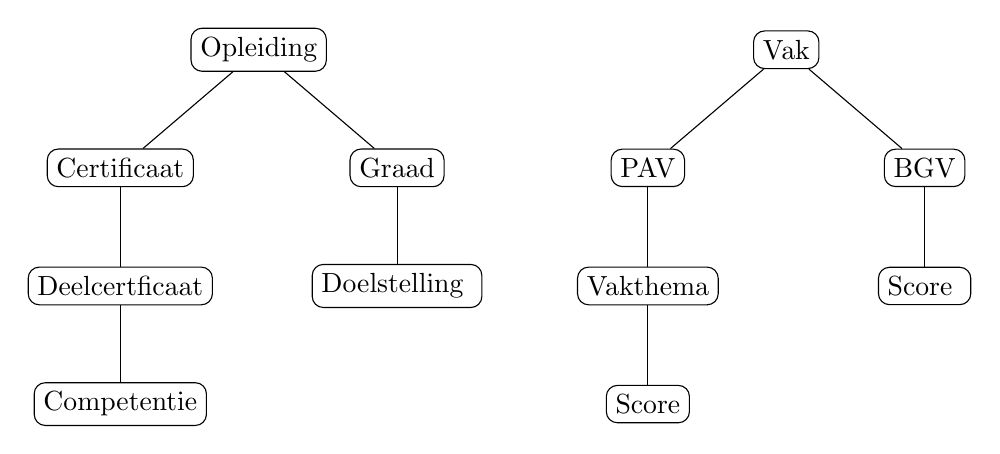
\begin{tikzpicture}[sibling distance=10em,
  every node/.style = {shape=rectangle, rounded corners,
    draw, align=center}]]
    
  \node {Opleiding}
    child { node {Certificaat} 
    	child { node {Deelcertficaat}  
    		child { node {Competentie} } 
    	} 
    }
    child { node {Graad}
      child { node {Doelstelling } } 
    };
    
    \node [draw] at (6.7, 0) {Vak}
    child { node {PAV} 
    	child { node {Vakthema}  
    		child { node {Score} } } }
    child { node {BGV}
      child { node {Score } } };
\end{tikzpicture}

\subsection{Modulo}
Modulo is een softwarepakket om gegevens over studenten bij te houden binnen scholen die het DBSO als onderwijsvorm toepassen. Het is echter geen algemeen beheersysteem; het bevat bijvoorbeeld geen functionaliteit om financiën te beheren. Wel houdt Modulo lijsten van klassen, aangeboden opleidingen en de voortgang van individuele studenten bij.

Modulo onderscheidt vier types gebruikers: beheerders, leerkrachten, studenten en ouders. Alle gebruikers hebben een webapplicatie ter beschikking waarin de volledige functionaliteit van het softwarepakket voor dat type gebruiker vertegenwoordigd is. Studenten en ouders hebben aanvullend toegang tot een Android applicatie, beschikbaar vanaf de Google Play Store.

Het softwarepakket bestaat uit zeven modules:

\begin{enumerate}
    \item \label{itm:mod_user_management} Gebruikersbeheer
    \item \label{itm:mod_course_management} Beheer van graden en certificaten
    \item \label{itm:mod_class_management} Klassenbeheer
    \item \label{itm:mod_grades_management} Puntenbeheer
    \item \label{itm:mod_student_progress} Voortgang van studenten
    \item \label{itm:mod_employer_management} Werkgeversbeheer
    \item \label{itm:mod_tasks} Taken
\end{enumerate}

Modules \ref{itm:mod_user_management} en \ref{itm:mod_class_management} zijn enkel beschikbaar voor beheerders. Alle overige modules zijn beschikbaar voor leerkrachten. Studenten en ouders beschikken enkel over modules \ref{itm:mod_student_progress} en \ref{itm:mod_tasks}. Modulo is dus veruit het meest uitgebreid voor leerkrachten. De volgende paragrafen geven een algemeen beeld van de functionaliteiten van de verschillende modules. Voor een gedetailleerde stap-voor-stap beschrijving van de acties die gebruikers moeten nemen om bepaalde taken uit te voeren, kan sectie \ref{sec:use_cases} geraadpleegd worden.

\newpage
Beheerders kunnen via module \ref{itm:mod_user_management} gebruikers toevoegen, verwijderen, bewerken en op actief of inactief zetten (wat hetzelfde effect heeft als een gebruiker verwijderen, met als verschil dat al diens gegevens bewaard blijven, waardoor de gebruiker later eenvoudig in zijn oorspronkelijke staat hersteld kan worden). Via module \ref{itm:mod_course_management} kunnen zij de eindtermen van de twee vakken binnen het DBSO, BGV en PAV, aanpassen. Beheerders kunnen ook certificaten binnen BGV op inactief zetten, wanneer deze niet door de school worden aangeboden.

Leerkrachten kunnen allereerst klassen samenstellen, binnen BGV of PAV, waaraan zij les geven (module \ref{itm:mod_class_management}). Vervolgens kunnen zij binnen deze klassen per lesdag punten (A,I,V) aan studenten toekennen, met toevoeging van commentaar (module \ref{itm:mod_grades_management}). Deze punten kunnen zij later ook opvragen in een scherm dat zowel algemene als gedetailleerde voortgang toont, of ze kunnen de punten in rapport vorm afdrukken (module \ref{itm:mod_student_progress}). Daarnaast kunnen leerkrachten de werkgeversdatabank, een lijst van alle werkgevers waar studenten hun praktijkdagen kunnen bij doorbrengen, bewerken, kunnen ze studenten aan werkgevers koppelen en kunnen ze contracten tussen deze studenten en werkgevers genereren, op basis van sjablonen, en deze afdrukken om te laten ondertekenen (module \ref{itm:mod_employer_management}). Tenslotte kunnen leerkrachten taken aan studenten toekennen en vervolgens de inzendingen van de studenten beoordelen (module \ref{itm:mod_tasks}).

Studenten en ouders kunnen respectievelijk hun eigen voortgang en die van hun kinderen bekijken (module \ref{itm:mod_student_progress}). Indien ouders meerdere kinderen op de school hebben, kunnen zij kiezen uit een lijst van kinderen om de voortgang van te bekijken. De voortgang kan bekeken worden zowel via de web- als via de mobiele applicatie. Hetzelfde geldt voor taken; studenten kunnen een inzending maken voor aan hen toegekende taken (enkel via de web applicatie) en zowel ouders als kinderen kunnen de status van alle toegekende taken bekijken (zowel via de web- als de mobiele applicatie) (module \ref{itm:mod_tasks}).



\newpage
\section{User requirements}  \label{sec:user_req}% voor de klant
\subsection{Functionele requirements}

\subsubsection{Gebruikersbeheer}
\begin{enumerate}[label=F\arabic*]
\item \label{itm:account_info} Het systeem moet toelaten om gebruikers toe te voegen, waarbij een account voor de gebruiker wordt aangemaakt. Hierbij moet de accountgerelateerde informatie\footnote{Dit zijn de rol (leerkracht, student, beheerder, ouder), e-mailadres, wachtwoord, voornaam en achternaam.} worden ingevuld. Een gebruiker moet ook verwijderd en bewerkt kunnen worden. Er moet ook een overzicht voorzien worden van alle gebruikers in het systeem.
\item \label{itm:student_info} Het systeem moet toelaten om voor een gebruiker met als rol `student' persoonlijke informatie\footnote{Deze info bestaat uit: geboortedatum, geboorteplaats, nationaliteit, rijksregisternummer, straat, nummer, bus, postcode, gemeente, gsm, telefoon ouders en rekeningnummer. We houden deze info alleen bij voor studenten omdat de school apart de gegevens van het personeel bijhoudt en we het telefoonnummer van de ouders bij de student bijhouden.} en inschrijvingsgerelateerde informatie\footnote{Dit is de info over hun opleiding, bestaande uit hun graad en certificaat.} in te vullen bij het aanmaken van de gebruiker, of aan te passen bij het bewerken van deze gebruiker.
\item Het systeem moet toelaten om (het account van) \'e\'en ouder te koppelen aan een student. Per student wordt dus hoogstens \'e\'en ouder-account voorzien. Als ouder kan men de voortgang van de student(en) waaraan die ouder gekoppeld is, bekijken.
\item Het systeem moet toelaten om in te stellen of een gebruiker al dan niet actief is. Een inactieve gebruiker komt niet meer voor in het systeem, maar alle persoonlijke info blijft beschikbaar. Daardoor kan de student zich niet meer aanmelden, en kunnen leerkrachten die student niet meer zien om er bv.\ een score aan toe te kennen. Indien later de gebruiker terug op actief gezet zou worden, moet men niet opnieuw alle info invullen\footnote{Ter motivatie hiervan vermelden we dat het in het deeltijds onderwijs voorvalt dat studenten zich gedurende hun opleiding uitschrijven. Maar dan later, wanneer bv. blijkt dat ze geen werk vinden, ze alsnog hun opleiding willen verder zetten.}.
\end{enumerate}

\subsubsection{Beheer van graden en certificaten}
\begin{enumerate}[label=F\arabic*,resume]
\item Het systeem moet een beheerder toelaten om de doelstellingen (binnen een graad) te bewerken. Er kunnen geen doelstellingen aangemaakt of verwijderd worden \footnote{De motivatie achter het manueel aanpassen van doelstellingen is dat deze doelstellingen door de overheid vaak moeilijk of onduidelijk verwoord zijn.}. Er moet een overzicht weergegeven kunnen worden van alle doelstellingen van een bepaalde graad.
\item Het systeem moet een beheerder toelaten om de competenties (binnen een deelcertificaat, binnen een certificaat) te bewerken. Er kunnen geen competenties aangemaakt of verwijderd worden. Er moet een overzicht weergegeven kunnen worden van alle certificaten. Voor een certificaat moet er een overzicht weergegeven worden van de deelcertificaten. Voor een deelcertificaat moet er een overzicht weergegeven kunnen worden van de competenties.
\item Het systeem moet toelaten om van een certificaat in te stellen of dit al dan niet door de school wordt aangeboden \footnote{De overheid lijst zo'n 150 certificaten op, maar een school zal er typisch slechts zo'n $20$ aanbieden}.
\end{enumerate}

\subsubsection{Klassenbeheer}
\begin{enumerate}[label=F\arabic*,resume]
\item Het systeem moet een leerkracht toelaten om een PAV-klas aan te maken, te verwijderen en te bewerken. De naam en graad moeten ingevuld worden. Ook moet het systeem een overzicht kunnen geven van alle PAV-klassen waar de leerkracht les aan geeft.
\item Het systeem moet een leerkracht toelaten om een BGV-klas aan te maken, te verwijderen en te bewerken. De naam en het certificaat moeten ingevuld worden. Ook moet het systeem een overzicht kunnen geven van alle BGV-klassen waar de leerkracht les aan geeft.
\item Het systeem moet een leerkracht toelaten om studenten aan een klas toe te voegen, een overzicht op te vragen van de studenten die in de klas zitten, en er studenten uit te verwijderen.
\item Het systeem moet een leerkracht toelaten om een vakthema voor een PAV-klas aan te maken, te verwijderen en te bewerken. De naam en beschrijving van het vakthema moeten ingevuld worden. Ook moet het systeem een overzicht kunnen geven van alle aangemaakte vakthema's. \footnote{Deze functie is niet mogelijk voor een BGV-klas.}
\item Het systeem moet een leerkracht toelaten om een remediëringsvakthema voor een aantal studenten van een PAV-klas aan te maken, te verwijderen en te bewerken. De naam en beschrijving van het remediëringsvakthema moeten ingevuld worden. Ook moet het systeem een overzicht kunnen geven van alle aangemaakte remediëringsvakthema's. \footnote{Deze functie is niet mogelijk voor een BGV-klas.}
\item Het systeem moet toelaten om doelstellingen aan een vakthema of remediëringsvakthema toe te voegen, een overzicht van de toegevoegde doelstellingen op te vragen, en er doelstellingen uit te verwijderen.
\item Het systeem moet toelaten om bij het aanmaken van een vakthema een bestaand vakthema in te laden, als een soort template. Alleen de vakthema's die tot dezelfde graad behoren als de graad van de klas waarvoor het vakthema aangemaakt wordt, kunnen gekozen worden. De naam, beschrijving en doelstellingen worden dan automatisch ingevuld voor het nieuwe vakthema.
\end{enumerate}

\subsubsection{Puntenbeheer}
\begin{enumerate}[label=F\arabic*,resume]
\item Het systeem moet toelaten om eenmalig een score (A,I,V) (zie woordenlijst) toe te kennen aan een doelstelling binnen een vakthema, voor een student. Ook moeten commentaar en de datum waarop de score behaald werd, ingesteld kunnen worden. Het systeem moet een overzicht kunnen geven van de toegekende score voor iedere doelstelling. De score, commentaar en datum moeten bewerkt kunnen worden.
\item Het systeem moet toelaten om meermaals een score (A,I,V) toe te kennen aan een competentie binnen een deelcertificaat, voor een student. Ook moeten commentaar en de datum waarop de score behaald werd, ingesteld kunnen worden. Het systeem moet een overzicht kunnen geven van de toegekende score voor iedere competentie. De score, commentaar en datum moeten bewerkt kunnen worden.
\item Het systeem moet toelaten om meerdere studenten gelijktijdig eenzelfde score (met eenzelfde commentaar en datum) toe te kennen. Dit is dus een multi-select. Ook voor het bewerken van scores (met commentaar en datum) moet deze multi-select mogelijk zijn.
\item Het systeem moet automatisch het behalen van een competentie of doelstelling blokkeren voor een student, indien deze reeds drie maal verworven (score V) werd.
\end{enumerate}

\subsubsection{Voortgang van studenten}
\begin{enumerate}[label=F\arabic*,resume]
\item Het systeem moet het verloop van het jaar kunnen weergeven per student voor PAV. Dit overzicht toont de behaalde score (A, I, V) per doelstelling per week. In totaal zijn er $38$ lesweken.
\item Het systeem moet het verloop van het jaar kunnen weergeven per student voor een deelcertificaat. Dit overzicht toont de behaalde score (A, I, V) per competentie (voor dat deelcertificaat) per week. In totaal zijn er $38$ lesweken.
\item Het systeem moet toelaten om een ingevuld rapport te genereren, voor een student. Ten eerste geeft dit aan hoeveel procent van de doelstellingen behaald (drie maal verworven) werden in de huidige graad (op het moment van het genereren van het rapport). Ten tweede geeft het rapport per deelcertificaat aan hoeveel procent van de competenties behaald werden. Ten derde geeft het rapport een algemeen overzicht, waarin wordt aangegeven hoeveel procent van de doelstellingen en competenties van alle graden en deelcertificaten samen behaald werden.
\item Het systeem moet loggen (timestamp bijhouden) wanneer een ouder of student de voortgang bekijkt. Als admin kan deze log opgevraagd worden. De log moet ook gewist kunnen worden \footnote{De motivatie hierachter is dat men de log aan het einde van het schooljaar niet meer nodig heeft.}.
\end{enumerate}

\subsubsection{Werkgeversbeheer}
\begin{enumerate}[label=F\arabic*,resume]
\item \label{itm:werkgever_info} Het systeem moet de beheerder toelaten om werkgevers waar de school mee samenwerkt toe te voegen \footnote{In het deeltijds onderwijs werkt een school vaak samen met bedrijven.}. Het systeem moet allerlei info bijhouden over de werkgever \footnote{Deze info bestaat uit de bedrijfsnaam, juridische vorm, BTW nummer, RSZ nummer, IPK nummer, PC nummer, erkenning PC, adres, telefoon, fax, email, rekeningnummer, naam en telefoon van de verantwoordelijke binnen het bedrijf.}. Een werkgever heeft geen account binnen Modulo, en dus geen toegang tot het systeem. Het systeem moet ook toelaten om een overzicht van alle werkgevers te geven, en een werkgever te bewerken of te verwijderen.
\item \label{itm:werkgever1} Het systeem moet toelaten aan een leerkracht om een werkgever (waar de school mee samenwerkt) aan een student toe te wijzen. Ook moet het systeem een overzicht kunnen geven dat per student de toegewezen werkgever toont (indien reeds een werkgever werd toegewezen). Een koppeling moet ook verwijderd kunnen worden.
\item Het systeem moet de beheerder toelaten om voor een werkgever in te stellen of er momenteel al dan niet een actieve samenwerking is. Dit houdt in dat de werkgever al dan niet door een leerkracht toegewezen kan worden aan een student (zie \ref{itm:werkgever1}). \footnote{De werkgever zal niet op ieder moment studenten kunnen te werk stellen.}
\item \label{itm:werkgever2} Het systeem moet toelaten om een contract te genereren voor de samenwerking tussen een student en werkgever. Het contract moet alle persoonlijke info over de student (zie \ref{itm:student_info}) en alle info over de werkgever (zie \ref{itm:werkgever_info}) bevatten. Het precieze uitzicht van het contract wordt in appendix \ref{vbContract} getoond.
\end{enumerate}

\subsubsection{Takenbeheer}
\begin{enumerate}[label=F\arabic*,resume]
\item Het systeem moet een leerkracht toelaten om een taak aan te maken, te verwijderen en te bewerken. De PAV-klas, naam van de taak, beschrijving en deadline van de taak moeten ingevuld worden. Ook moet het systeem een overzicht kunnen geven dat alle aangemaakte taken toont. \footnote{Deze functie is niet mogelijk voor een BGV-klas.}
\item Het systeem moet een student toelaten om één bestand te uploaden als oplossing voor een taak.
\item Het systeem moet een student toelaten om een overzicht op te vragen van alle taken waar hij/zij nog geen oplossing voor heeft geüpload.
\item Het systeem moet een ouder toelaten om een overzicht op te vragen van alle taken waar zijn/haar kind nog geen oplossing voor heeft geüpload.
\item Het systeem moet een leerkracht toelaten om voor een taak een overzicht op te vragen dat per leerling aangeeft of deze reeds een oplossing geüpload heeft, en welke score de leerkracht gaf (indien reeds een score gegeven werd).
\item Het systeem moet een leerkracht toelaten om alle geüploade oplossingen voor een taak te downloaden. Dit zowel één voor één, als in één zip-bestand die alle taken bundelt.
\item Het systeem moet een leerkracht toelaten om een student een score (A,I,V) te geven op een geüploade oplossing. Hierbij kan (optioneel) een korte commentaar geschreven worden. De score en commentaar moeten ook bewerkt kunnen worden.
\item Het systeem moet toelaten om meerdere studenten gelijktijdig eenzelfde score en commentaar toe te kennen. Dit is dus een multi-select. Ook voor het bewerken van de score en commentaar moet deze multi-select mogelijk zijn.
\end{enumerate}

% extra's worden in 'systeemevolutie' besproken

\subsection{Usability}
De gebruikersinterface is een uitgesproken belangrijk onderdeel van Modulo, want aangezien het om een managementsysteem gaat, staat of valt de bruikbaarheid van het softwarepakket met diens overzichtelijkheid. Voor alle types gebruikers zijn duidelijkheid en een vlotte werking essentieel, omdat ze vaak met lange lijsten van complexe gegevens werken, zoals de lijst van scores die een student behaald heeft, of de lijst van studenten in een klas. Ook consistentie is van belang, in het bijzonder omdat er zowel een web- als een mobiele applicatie beschikbaar is. Deze zijn eenvoudiger afwisselend te gebruiken indien hun design en werking vergelijkbaar zijn.

Om een vlotte werking te bevorderen, kunnen meerdere items tegelijk uit lijsten geselecteerd worden, waarna acties op alle geselecteerde items tegelijk kunnen worden uitgevoerd (bv. een score voor een bepaalde doelstelling of competentie kan aan meerdere studenten, of zelfs een hele klas, tegelijk worden toegekend). Ook biedt een zoekfunctie de mogelijkheid om snel specifieke items in een lijst terug te vinden.

Consistentie wordt bereikt door middel van eenzelfde design (kleurenschema, fonts en ontwerp van elementen) over de gehele web- en mobiele applicatie heen. Ook een consistente woordkeuze (bv. voortgang van studenten wordt steeds `voortgang' genoemd en niet soms `punten' of `resultaten') en een consistente layout (bv. knoppen om items in een lijst te bewerken, toe te voegen of te verwijderen kunnen steeds in dezelfde plaats gevonden worden, of het nu om punten voor een vak of studenten in een klas gaat) dragen hiertoe bij.

Modulo voorziet voor iedere graad reeds de bijhorende doelstellingen, opgelegd door de overheid. Ook voorziet Modulo reeds alle certificaten die door de overheid erkend zijn. De bijhorende deelcertificaten, met hun bijhorende competenties, worden ook voorzien. Hierdoor moet de admin al deze info niet meer zelf invullen bij het in gebruik nemen van Modulo.

\todo[inline]{usability: gebruiksvriendelijke aanpak van vakthemas}

\subsection{Reliability}
Zowel de web- als de mobiele applicatie zijn slechts interfaces naar de back-end. Bijgevolg is uptime van de back-end servers essentieel voor de reliability van het softwarepakket. Om die reden wordt hosting van deze servers uitbesteed aan een gespecialiseerd bedrijf met een hoge uptime garantie, dat deze taak vermoedelijk goedkoper en betrouwbaarder kan uitvoeren dan het ontwikkelingsteam zelf.


\subsection{Performance}
Op het vlak van performantie zijn er geen specifieke vereisten, maar een vlotte werking van het softwarepakket is uiteraard belangrijk. Daarom moeten lange responstijden en merkbare laadtijden tot een minimum beperkt worden. Het ontwikkelingsteam profileert de performantie en voert optimalisaties door waar nodig en mogelijk. 
% Deze tijd was onmogelijk, dus beter weglaten, als we dit nu toch niet kunnen waarmaken?
% Volgens het RAIL performantie model \cite{RAIL}, moeten performantievertragingen beperkt worden tot 300ms - 1000ms. De gebruiker ervaart dan natuurlijke en progressieve voortgang van taken.


\subsection{Supportability}
Het softwarepakket moet makkelijk uitbreidbaar en eenvoudig te onderhouden zijn. In het geval van een onderwijshervorming moeten bijvoorbeeld met weinig moeite nieuwe certificaten, doelstellingen en competenties kunnen worden toegevoegd (of verwijderd). De back-end van het softwarepakket draait op servers van een gespecialiseerd hosting bedrijf en blijft zo eenvoudig toegankelijk voor het ontwikkelingsteam, en de mobiele applicatie wordt geïnstalleerd vanaf de Google Play Store, waardoor ook daar eenvoudig updates doorgevoerd kunnen worden.


\subsection{Legal}
Het softwarepakket moet voldoen aan de privacy wetgeving, in het bijzonder betreffende de resultaten en persoonlijke informatie van de studenten. Ouders mogen enkel de gegevens van hun eigen kinderen kunnen bekijken en enkel aangemelde personeelsleden mogen gevoelige informatie, waaronder ook de rekeningnummers van studenten en werkgevers, kunnen opvragen.

De back-end van het softwarepakket draait op servers van een gespecialiseerd hosting bedrijf dat volledige privacy en een goede beveiliging garandeert, zowel fysiek als virtueel. Verbindingen tussen de back-end server en de web- of mobiele applicatie gebeuren steeds over HTTPS en bevatten steeds een ID om de identiteit van de gebruiker kenbaar te maken.

Het softwarepakket hoeft geen rekening te houden met de wetgeving rond contracten. Deze kunnen enkel gegenereerd worden vanaf sjablonen en vervolgens afgeprint, maar worden niet digitaal ondertekend noch opgeslagen.


\subsection{Operations}
Na de ingebruikname van Modulo worden de doelstellingen en competenties up-to-date gehouden. Concreet betekent dit het volgende: de overheid zou competenties (van een certificaat) of doelstellingen (van een graad) kunnen aanpassen, verwijderen of toevoegen. Ook zou de overheid een nieuw certificaat kunnen opstellen (met bijhorende competenties). Modulo zal zulke wijzigingen op maandelijks basis voor de klant updaten.


\section{Systeemarchitectuur}  \label{sec:systeemarchitectuur} % NIET voor de klant
Het softwarepakket bestaat uit 3 deelsystemen:

\begin{enumerate}
    \item Een centrale back-end, onzichtbaar voor de gebruiker.
    \item Een front-end als webapplicatie.
    \item Een front-end als mobiele applicatie.
\end{enumerate}

\begin{figure}[H]
  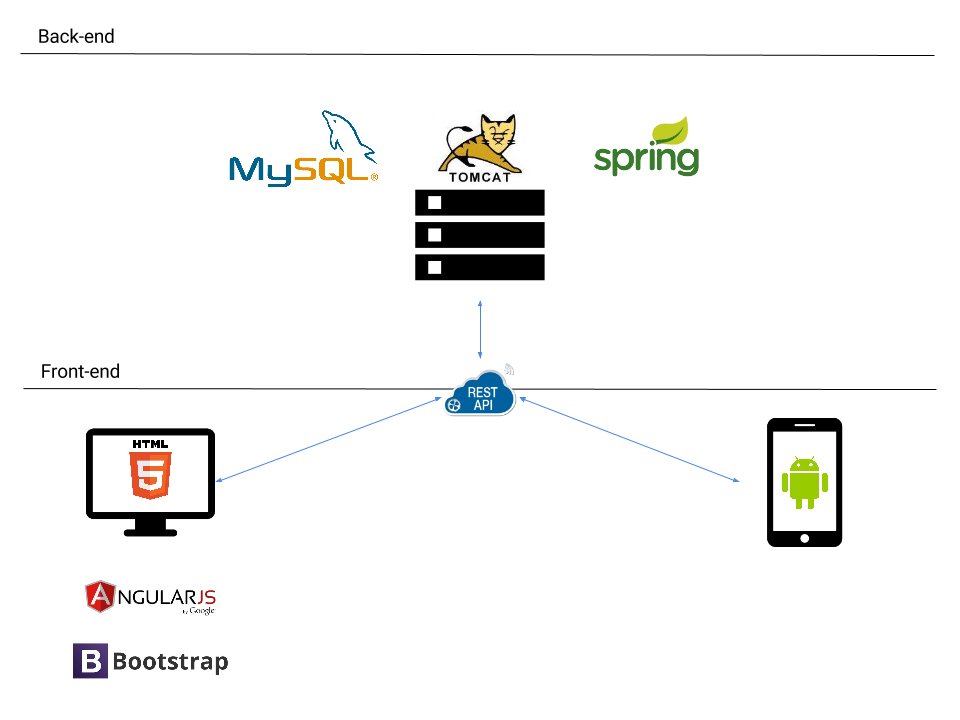
\includegraphics[width=\textwidth]{technologie_stack}
  \caption{Systeemarchitectuur}
  \label{fig:Systeemarchitectuur}
\end{figure}

De back-end wordt geïmplementeerd in Java, met behulp van het \textit{Spring Framework} \cite{Spring}. Voor de webapplicatie worden het \textit{AngularJS Framework} \cite{AngularJS} en het \textit{Bootstrap Framework} \cite{Bootstrap} gebruikt. De mobiele applicatie is beschikbaar voor het Android platform en wordt opnieuw in Java geïmplementeerd. De interactie tussen de front-end en back-end gebeurt door middel van zogenoemde \textit{RESTful} communicatie \cite{REST}. MySQL \cite{MySQL} wordt gebruikt als databasemanagementsysteem en wordt samen met de back-end gehost op een \textit{Tomcat} \cite{Tomcat} server.\todo{Zin toegevoegd, klant + gratis = goed?} Deze technologie stack kan op vele systemen gratis geïnstalleerd worden.

\newpage
\subsection{Motivatie}
\begin{description}
    \item[Java] We wensen gebruik te maken van een programmeertaal die zich uitstekend leent voor business logica en veel gebruikt wordt in het enterprise landschap. De twee programeertalen die hiervoor typisch gebruikt worden zijn C\# en Java, waarbij onze keuze valt op Java. Eén van de voordelen van deze taal is het cross-platform karakter. Een bijkomend voordeel is dat Java beschikt over een uitgebreid aantal frameworks en bibliotheken die ontwikkeling vergemakkelijkt. Het is een robuuste en veel gebruikte taal die al meer dan 20 jaar wordt gebruikt en waar periodiek een nieuwe versie van worden uitgebracht door \textit{Oracle}. Ze is backwards compatible: oudere code werkt nog steeds op nieuwere versies van de \textit{Java Virtual Machine}.
    
    \item[MySQL] \todo{veranderen door PostresSQL} is een vrij te gebruiken relationeel database-managementsysteem, beheerd door \textit{Oracle}. Het systeem is al lang op de markt en heeft zich al meermaals bewezen. Het is een wijd geadopteerd systeem dat door vele bedrijven gebruikt wordt, onder andere door Smartschool. In vergelijking met andere database systemen, zoals Postgres, is het trager voor complexere queries, maar sneller voor eenvoudige queries. Omdat ons systeem juist enkel gebruik maakt van eenvoudige queries, is MySQL een goede keuze. 
    
    \item[Spring Framework] is een antwoord op de kritiek die gericht is aan de werking van het klassieke Java EE. Eén van de grote sterktes is de uitgebreide documentatie. Met behulp van Spring is men in staat om snel een API te ontwikkelen. Ook hebben we het Jersey Framework overwogen, maar kozen we toch voor Spring wegens alle andere extra componenten die het framework te bieden heeft (o.a. Spring Web, Spring Security en Spring Data).
    
    \item[AngularJS] is een JavaScript framework dat is ontwikkeld en voornamelijk wordt onderhouden door Google. Dit framework kende in de afgelopen jaren een explosieve groei en werd immens populair voor de ontwikkeling van \textit{single page applications}. Het grote voordeel van AngularJS ten opzichte van het tradionele JavaScript is de mogelijkheid tot een snellere ontwikkeling. Ook biedt het framework uitstekende mogelijkheden voor testing, dat de kwaliteit van het product alleen ten goede komt. \todo{Nog iets zeggen over versie 2 of enkel op de verdediging?}

    \item[Bootstrap CSS] is een van de meest populaire CSS frameworks, ontwikkeld door Twitter, dat gebruikt wordt voor de ontwikkeling van responsieve webapplicaties. Voordelen zijn de vereenvoudigde en versnelde ontwikkeling, consitentie van de look-and-feel. Webpagina's met Bootstrap zijn \textit{responsive} out-of-the-box, d.w.z. dat de webpagina zich automatisch aanpast aan de grote van het beeldscherm.
    Bootstrap maakt gebruik van JQuery, een andere JavaScript framework dat niet compatibel is met AngularJS. Om toch alle voordelen te kunnen gebruiken van Bootstrap, kan er gebruik gemaakt worden van de eenvoudige Angular-UI \cite{AngularUI} Bootstrap bibliotheek.
    \todo{Jquery en Angular en compatibility misschien nog wat toelichten.}
\end{description}



\clearpage
\section{Use cases} \label{sec:use_cases}

%%%%%%%%%%%%%%%%%%%%%%%%%%%%%%%%%%%%%%%%%%%%%%%%%%%%%%%%%%%%%%%%%%%%%%%%%%%%%
%BEHEERDER
%%%%%%%%%%%%%%%%%%%%%%%%%%%%%%%%%%%%%%%%%%%%%%%%%%%%%%%%%%%%%%%%%%%%%%%%%%%%%

In alle use cases die in dit sectie voorkomen geldt de preconditie dat de leerkracht aangemeld is.

\subsection{Beheerder}
%Gebruikers toevoegen
\begin{usecase}
    \addtitle{Use Case 1}{Gebruiker toevoegen} 
    \additemizedfield{Primaire actor}{
    	\item Beheerder
    } 
    \additemizedfield{Stakeholders en interests}{ 
        \item Beheerder: Andere mensen toegang geven tot het systeem.
        \item Student: De student krijgt toegang tot het systeem.
        \item Leerkracht: De leerkracht krijgt toegang tot het systeem.
        \item Ouder: De ouder krijgt toegang tot het systeem.
    }
    \addfield{Preconditie}{
        De certificaten en graden moeten bestaan.
    }
    \addfield{Postconditie}{
        De gegevens over de gebruiker worden correct opgeslagen.
    }
    \addscenario{Hoofdscenario}{
        \item Beheerder kiest ``Gebruikersbeheer''.
        \item Het systeem geeft een lijst weer van alle gebruikers.
        \item Beheerder kiest ``Toevoegen''.
        \item Systeem toont een dropdown waarmee de gebruikersrol dient ingesteld te worden, deze staat default op student.
        \item Beheerder kiest ``student''  als gebruikersrol.
        \item Systeem toont een leeg formulier waarin alle informatie over de student moet worden ingevuld. Dit zijn de persoonlijke, accountgerelateerde en inschrijvingsgerelateerde informatie (zie \ref{itm:student_info}, \ref{itm:account_info} en \ref{itm:student_info} ).
        \item Beheerder vult alle benodigde informatie in.
        \item Beheerder bevestigt ingevulde informatie door op ``Aanmaken'' te klikken.
        \item Systeem toont de aangepaste lijst met gebruikers.
    }   
    \addscenario{Alternatieve scenarios}{
        \item[5.a] Beheerder kiest ``leerkracht'' als gebruikersrol.
        \item[5.b] Beheerder kiest ``beheerder'' als gebruikersrol.
        \item[5.c] Beheerder kiest ``ouder'' als gebruikersrol.
        \item[6.a-c] Alleen accountgerelateerde info moet ingevuld worden.
        \item[9.a] Foutieve gegevens: Systeem behoudt de huidige pagina en geeft een error message bij de foutieve informatie (user bestaat al, verkeerd formaat email of rekeningnummer).
    }
    \addfield{Frequentie van voorkomen}{
        Op dagen waarop studenten zich in de school kunnen inschrijven, zal deze functie meermaals per dag gebruikt worden. Buiten deze periode wordt de functionaliteit amper gebruikt.
    }
\end{usecase}


\todo{nakijken}
% Gebruikers wijzigen
\begin{usecase}
    \addtitle{Use Case 2}{Gebruiker bewerken} 
    \additemizedfield{Actoren}{
    	\item Beheerder
    }
    \addscenario{Beschrijving}{
        \item[] \textbf{Hoofdscenario:} \\
        Beheerder kiest ``Gebruikersbeheer''. Het systeem geeft een lijst weer van alle gebruikers. Hier kan de beheerder kiezen om een gebruiker te bewerken door op het icoon te klikken. 
        De gebruiker kiest voor bewerken. Systeem toont een formulier waar alle   inschrijvingsgerelateerde informatie (zie \ref{itm:student_info}, \ref{itm:account_info} en \ref{itm:student_info}) reeds ingevuld is van de geselecteerde gebruiker. Deze info kan hier aangepast worden. De beheerder klikt op de knop ``Opslaan''.
    }
\end{usecase}

\todo{nakijken}
% Gebruikers verwijderen
\begin{usecase}
    \addtitle{Use Case 3}{Gebruiker verwijderen} 
    \additemizedfield{Actoren}{
    	\item Beheerder
    }
    \addscenario{Beschrijving}{
        \item[] \textbf{Hoofdscenario:} \\
        Beheerder kiest ``Gebruikersbeheer''. Het systeem geeft een lijst weer van alle gebruikers. Hier kan de beheerder kiezen om een gebruiker te verwijdere door op het icoon te klikken. 
        De gebruiker kiest voor verwijderen. Systeem toont een pop-up met de vraag of de geselecteerde gebruiker zeker verwijderd wil worden. Beheerder klikt op de knop ``Bevestigen''.
        \item[] \textbf{Alternatieve scenarios:} \\
        De beheerder kan in de pop-up de actie annuleren door op de knop ``Annuleren'' te klikken.
    }
\end{usecase}


\todo{nakijken}
% Certificaten beheren (actief/inactief)
\begin{usecase}
    \addtitle{Use Case 4}{Certificaten beheren} 
    \additemizedfield{Actoren}{
    	\item Beheerder
    }
    \addscenario{Beschrijving}{
        \item[] \textbf{Hoofdscenario:} \\
        Beheerder gaat naar het menu ``Certificaten''. Het systeem toont een lijst van alle certificaten. Achter ieder certificaat staat een icoon dat aanduidt of het certificaat actief of inactief staat. De beheerder scrollt tot hij het gewenste certificaat tegenkomt en klikt op het icoon. Het systeem toont een pop-up dat bevestiging vraagt. De beheerder klikt op ``Bevestigen''.
        \item[] \textbf{Alternatief scenario:}\\
        In plaats van te scrollen tot het gewenste certificaat gevonden is, zoekt de beheerder het certificaat aan de hand van een zoekbalk.\\
        In plaats van akkoord te gaan met de wijziging, klikt de beheerder op ``Annuleer''.
    }
\end{usecase}


\todo{nakijken}
% Competenties (BGV) beheren
\begin{usecase}
    \addtitle{Use Case 5}{Competenties beheren} 
    \additemizedfield{Actoren}{
    	\item Beheerder
    }
    \addscenario{Beschrijving}{
        \item[] \textbf{Hoofdscenario:} \\
        Beheerder gaat naar het menu ``Opleidingen beheren''. Men kiest voor ``Competenties''. Het systeem toont een tree-view van de certificaten, waaronder de deelcertificaten staan, waaronder de competenties staan. De beheerder klikt het benodigde certificaat open, klikt het benodigde deelcertificaat open en klikt dan op het bewerk icoon van de competentie. Het systeem toont de beschrijving van de gekozen competentie. De beheerder bewerkt de informatie en klikt op ``Opslaan''.
        \item[] \textbf{Alternatief scenario:} \\
    	In plaats van certificaat en deelcertificaat open te klappen, kan er ook gezocht worden naar certificaten, deelcertificaten en competenties aan de hand van een zoekbalk.    
      	}
\end{usecase}



% Doelstellingen (PAV) beheren
\todo{nakijken}
\begin{usecase}
    \addtitle{Use Case 6}{Doelstellingen beheren} 
    \additemizedfield{Actoren}{
    	\item Beheerder
    }
    \addscenario{Beschrijving}{
        \item[] \textbf{Hoofdscenario:} \\
        Beheerder gaat naar het menu ``Opleidingen beheren''. Men kiest voor ``Doelstellingen''. Het systeem toont een tree-view van de graden, waaronder de doelstellingen staan. De beheerder klikt de benodigde graad open en klikt dan op het bewerk icoon van de doelstelling. Het systeem toont de beschrijving van de gekozen doelstelling. De beheerder bewerkt de informatie en klikt op ``Opslaan''.
        \item[] \textbf{Alternatief scenario:} \\
    	In plaats van graad open te klappen, kan er ook gezocht worden naar doelstellingen aan de hand van een zoekbalk.    
      	}
\end{usecase}

\todo{usecase diagram updaten?}
\begin{figure}[H]
  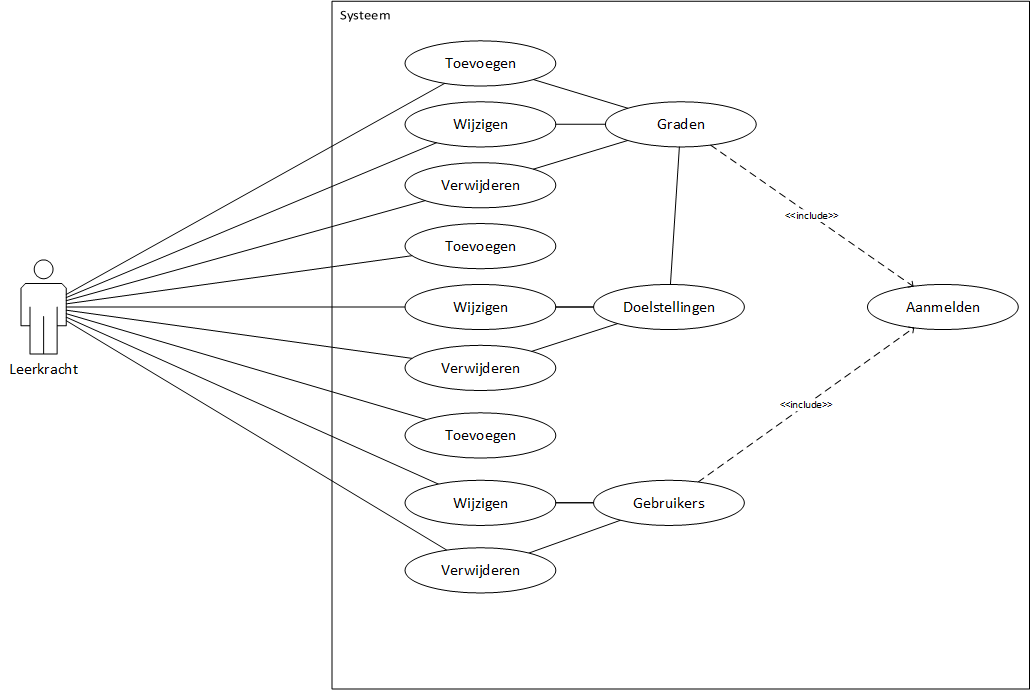
\includegraphics[width=\textwidth]{uc_beheerder}
  \caption{Usecase diagram voor de beheerder}
  \label{fig:usecase_beheerder}
\end{figure} 



%%%%%%%%%%%%%%%%%%%%%%%%%%%%%%%%%%%%%%%%%%%%%%%%%%%%%%%%%%%%%%%%%%%%%%%%%%%%%
%LEEKRACHT
%%%%%%%%%%%%%%%%%%%%%%%%%%%%%%%%%%%%%%%%%%%%%%%%%%%%%%%%%%%%%%%%%%%%%%%%%%%%%
\vspace{3em}
\subsection{Leerkracht}

In alle use cases die in dit sectie voorkomen geldt de preconditie dat de leerkracht aangemeld is.

\todo{nakijken}
% Werkgevers toevoegen
\begin{usecase}
    \addtitle{Use Case 7}{Werkgevers toevoegen} 
    \additemizedfield{Actoren}{
    	\item Leerkracht
    }
    \addscenario{Beschrijving}{
        \item[] \textbf{Hoofdscenario:} \\
		Leerkracht  kiest ``Werkgeversbeheer''. Systeem toont lijst van werkgevers. De beheerder klikt op de knop ``Toevoegen''. Het systeem toont een formulier waarin de werkgever info ingevuld kan worden (zie \ref{itm:werkgever_info}). De leerkracht vult alle informatie in en klikt op ``Toevoegen''.
	}
\end{usecase}

\todo{nakijken}
% Werkgevers bewerken
\begin{usecase}
    \addtitle{Use Case 8}{Werkgevers bewerken} 
    \additemizedfield{Actoren}{
    	\item Leerkracht
    }
    \addscenario{Beschrijving}{
        \item[] \textbf{Hoofdscenario:} \\
		Leerkracht  kiest ``Werkgeversbeheer''. Systeem toont lijst van werkgevers. De beheerder klikt op het bewerk icoon dat achter iedere werkgever staat. Het systeem toont een formulier waarin de werkgever info ingevuld staat (zie \ref{itm:werkgever_info}). Hier bewerkt de leerkracht de info. De leerkracht vult alle informatie in en klikt op ``Opslaan''. Het systeem toont een pop-up met de vraag of de gebruiker zeker is om de gewijzigde info op te slaan. De leerkracht klikt op de knop ``Bevestigen''.
		\item[] \textbf{Alternatief scenario:} \\
		In plaats van te bevestigen annuleert de leerkracht het opslaan van de gewijzigde info door op de knop ``Annuleren'' te klikken.
	}
\end{usecase}

\todo{nakijken}
% Werkgevers bewerken
\begin{usecase}
    \addtitle{Use Case 8}{Werkgevers bewerken} 
    \additemizedfield{Actoren}{
    	\item Leerkracht
    }
    \addscenario{Beschrijving}{
        \item[] \textbf{Hoofdscenario:} \\
		Leerkracht  kiest ``Werkgeversbeheer''. Systeem toont lijst van werkgevers. De beheerder klikt op het verwijder icoon dat achter iedere werkgever staat. Het systeem toont een pop-up met de vraag of de gebruiker zeker is om de werkgever te verwijderen. De leerkracht klikt op de knop ``Bevestigen''.
		\item[] \textbf{Alternatief scenario:} \\
		In plaats van te bevestigen annuleert de leerkracht het verwijderen van de werkgever door op de knop ``Annuleren'' te klikken.
	}
\end{usecase}

% Werkgever koppelen
\begin{usecase}
    \addtitle{Use Case 9}{Werkgever koppelen} 
    \additemizedfield{Actoren}{
    	\item Leerkracht
    }
    \addscenario{Beschrijving}{
        \item[] \textbf{Hoofdscenario:} \\
		De Leerkracht gaat naar ``Werkgever toewijzen'' binnen het menu ``Werkgeversbeheer''. Het systeem toont een lijst met de werkgevers en de student waaraan deze gekoppeld is. De leerkracht kiest om een nieuwe koppeling toe te voegen. Men zoekt en selecteert de gewenste student en de gewenste werkgever, en klikt op de knop ``Koppelen''.\\
    }
\end{usecase}

% Contract genereren
\begin{usecase}
    \addtitle{Use Case 10}{Contract genereren} 
    \additemizedfield{Actoren}{
    	\item Leerkracht
    }
    \addscenario{Beschrijving}{
        \item[] \textbf{Hoofdscenario:} \\
          Leerkracht meldt zich aan via de webapplicatie. De Leerkracht gaat naar ``Contracten'' in het menu ``Werkgeversbeheer''. Het type contract wordt gekozen alsook de student waar een contract voor moet worden opgesteld. De leerkracht klikt op de knop ``Genereer contract''. Info over de student en de werkgever worden automatisch ingevuld in het contract. Het contract wordt automatisch in pdf formaat gedownload. \\
        \item[] \textbf{Alternatieve scenarios:} \\
        Er werd geen werkgever aan de student toegewezen (Use Case 5). De leerkracht krijgt hier een melding van, maar het contract wordt wel gegenereerd (zonder de informatie over de werkgever).\\
    }
\end{usecase}


\todo{Puntenbeheer bespreken in groep en fixen}
% Puntenbeheer 
\begin{usecase}
    \addtitle{Use Case 11}{Puntenbeheer} 
    \additemizedfield{Primaire actor}{
    	\item Leerkracht
    } 
    \additemizedfield{Stakeholders en interests}{ 
        \item Leerkracht: Wilt een student op een gemakkelijke manier een score geven op een competentie/doelstelling.
    }
    \addfield{Preconditie}{
        De leerkracht moet aangemeld zijn. De graden, certificaten, klassen en studenten moeten bestaan.
    }
    \addfield{Postconditie}{
        De punten zijn opgeslagen. De aanpassing wordt weergegeven in de voortgang van de student. Doelstelling die drie keer is verworven, wordt in het grijs gezet wanneer er op een andere dag punten worden gegeven.}
    \addscenario{Hoofdscenario}{
        \item Leerkracht  kiest ``Puntenbeheer''.
        \item De leerkracht kiest in de eerste dropdown voor BGV.
        \item De leerkracht kiest in de tweede dropdown het certificaat.
        \item De leerkracht kiest in de derde dropdown de klas.
        \item De leerkracht kiest in de vierde dropdown de deelcertificaat.
        \item De leerkracht kiest op welke dag de competenties geëvalueerd werden.
        \item Het systeem toont een matrix met aan de linkerzijde de competenties die bij het gekozen deelcertificaat horen, en met bovenaan de studenten uit de gekozen klas. 
        \item De leerkracht selecteert de cel van de matrix die overeenkomt met de competentie en student waaraan hij een scoren wil geven.
        \item Onder de matrix toont het systeem een dropdown om de score (A, I, V) te geven en een veld om commentaar te schrijven (ter motivatie van de toegekende score).
        \item De leerkracht kiest in het dropdown A, I, V of leeg (als er geen score is gegeven).
        \item De leerkracht typt commentaar om de score te motiveren.
        \item De leerkracht klikt op ``Opslaan''.
        \item Het systeem behoudt de huidige pagina en de geselecteerde cel in het matrix wordt gedeselecteerd.
    }   
    \addscenario{Alternatieve scenarios}{
        \item[2.a] PAV: De leerkracht kiest voor PAV.
        \item[3.a] PAV: De leerkracht kiest voor de graad waarin hij een bepaalde klas wilt.
        \item[5.a] PAV: De leerkracht kiest voor het vakthema dat hij wilt beoordelen.
        \item[6.a] PAV: De leerkracht kiest op welke dag de doelstellingen geëvalueerd werden.
        \item[6.b] Score wijzigen: De leerkracht kiest de dag waarop hij de te wijzigen score gaf.
        \item[7.a] PAV: Het systeem geeft een matrix weer met aan de linkerzijde de doelstellingen die bij het gekozen vakthema horen, en met bovenaan de studenten uit de gekozen klas. 
        \item[7.b] Reeds beoordeelde doelstelling binnen een vakthema: De matrix wordt op bijna dezelfde manier weergegeven. Het enige verschil is dat de cel overeenkomstig met de reeds beoordeelde doelstelling is grijs gemaakt. Alleen op de dag waarop de score werd gegeven, is dit niet zo en kan de score dus worden gewijzigd.
        \item[7.c] Reeds behaalde doelstelling/competentie: De cel overeenkomstig met een doelstelling/competentie die de student reeds behaald (= drie keer verworven) heeft, is grijs. Enkel op de dagen dat ``V'' (verworven) als score werd toegekend, is dit niet het geval en kan de score dus gewijzigd worden.
        \item[8.a] Meerdere studenten en competenties/doelstellingen eenzelfde score en commentaar geven: De leerkracht selecteert alle gewenste cellen en vult onderaan de gemeenschappelijke score en commentaar in.
        \item[9.a] Verkeerde student punten gegeven: Selecteer de lege optie in de dropdown en deselecteer de cel in de matrix.
    }
    \addfield{Frequentie van voorkomen}{
        Bijna iedere dag dat er les wordt gegeven (2 keer per week)
    }
\end{usecase}

% !!!!!!!!!!! als je op een punt klikt krijg je een vakje met de commentaar te zien en voor pav het vakthema
% !!!!!!!!!!! toch nie mogelijk maken om in de voortgang punten aan te passen ? anders moet ge gaan kijken welke dag behaald en dan terug naar punten geven gaan wat veel stappen zijn
% Voortgang studenten (+rapporten)
\todo{Voortgang studenten bespreken in groep en fixen}
\begin{usecase}
    \addtitle{Use Case 12}{Voortgang studenten} 
    \additemizedfield{Actoren}{
    	\item Leerkracht
    }
    \addscenario{Beschrijving}{
        \item[] \textbf{Hoofdscenario:} \\
        Leerkracht meldt zich aan via de webapplicatie. Leerkracht  kiest ``Voortgang studenten''. De leerkracht krijgt een lijst van klassen waar hij les aan geeft. Hij kiest een klas en vervolgens een student uit de klas waar hij de voortgang van wilt zien. De voortgang voor BGV en PAV staan in aparte tabs. De voortgang is een wekelijks overzicht van wanneer competenties(BGV)/doelstellingen(PAV) behaald zijn door deze student.\\
        \item[] \textbf{Alternatieve scenarios:} \\
        De leerkracht kan per student een rapport bekijken en dit afdrukken (in pdf formaat). Het rapport geeft een algemeen beeld van hoe de student het gedaan heeft a.d.v. staafdiagrammen (Per deelcertificaat/vakthema hoeveel competenties/doelstellingen ingeoefend en verworven zijn uit een totaal aantal te behalen competenties/doelstellingen).
    }
\end{usecase}

\todo{use case nummering verhogen vanaf hier}
\todo{evt fully dressed use-case}
% Klasbeer
\begin{usecase}
    \addtitle{Use Case 9}{Klasbeheer} 
    \additemizedfield{Actoren}{
    	\item Leerkracht
    }
    \addscenario{Beschrijving}{
        \item[] \textbf{Hoofdscenario:} \\
        Leerkracht meldt zich aan via de webapplicatie. Leerkracht kiest ``Mijn klassen''. Het systeem toont een lijst van klassen waaraan de leerkracht les geeft. De leerkracht kan hier klassen toevoegen, wijzigen en verwijderen. De leerkracht kiest om een BGV- of PAV-klas te wijzigen. De leerkracht kiest om een PAV-klas te wijzigen. Het systeem toont een lijst van studenten in de tab ``Studenten''. De leerkracht klikt op de knop ``Toevoegen''. De leerkracht kiest een graad onder welke deze klas behoort via een dropdown (automatisch ingevuld met de huidige graad waaronder deze klas behoort). Het systeem toont een tree-view van studenten binnen deze graad onderverdeeld per certificaat waartoe ze behoren. De leerkracht kan een enkele student toevoegen door deze aan te vinken maar kan ook een certificaat aanvinken, alle studenten onder de certificaat worden dan toegevoegd aan de klas. (De leerkracht kan zo bv. alle studenten die ingeschreven zijn in de 2de graad en in het certificaat Metselaar toevoegen aan zijn klas).
        \item[] \textbf{Alternatie scenarios:} \\
        De leerkracht kiest om een BGV-klas te wijzigen. Het systeem toont een lijst van studenten in de tab ``Studenten''. De leerkracht klikt op de knop ``Toevoegen''. De leerkracht kiest een certificaat onder welke deze klas behoord via een dropdown (automatisch ingevuld met de huidige certificaat waaronder deze klas behoort). Het systeem toont een tree-view van studenten binnen de gekozen certificaat met het certificaat als root. De leerkracht kan studenten toevoegen op dezelfde manier als bij een PAV-klas. (De leerkracht kan zo bv. alle studenten die ingeschreven zijn voor het certificaat Metselaar toevoegen aan zijn klas).
    }
\end{usecase}

\todo{Remediëringstaak aparte use case}
%Klasbeheer -  Vakthema's
\begin{usecase}
    \addtitle{Use Case 10}{Klasbeheer -  Vakthema's} 
    \additemizedfield{Actoren}{
    	\item Leerkracht
    }
    \addscenario{Beschrijving}{
        \item[] \textbf{Hoofdscenario:} \\
        Leerkracht navigeert naar zijn klassen (Use case 9). De leerkracht kiest om een PAV-klas te wijzigen. De leerkracht selecteert de tab ``Vakthema's''. Het systeem toont een lijst van vakthema's. De leerkracht kan een vakthema toevoegen, verwijderen of wijzigen.
        \begin{itemize}
            \item[1] De leerkracht kiest om een nieuw vakthema toe te voegen. Het systeem toont een textbox voor de in te vullen vaknaam en een lijst van alle doelstellingen. Naast iedere doelstelling staat een tellertje dat aangeeft hoe vaak deze doelstelling reeds aan een vakthema werd toegekend \footnotemark. De leerkracht vinkt de doelstellingen aan die aangeboden moeten worden binnen dit vakthema.
            \item[2] De leerkracht kiest om een vakthema te wijzigen. De gegevens wijzigen werkt analoog met het toevoegen van een nieuw vakthema.
            \item[3] De leekracht kiest om een vakthema te verwijderen. Het systeem verwijdert het gekozen vakthema.
        \end{itemize}
        \item[] \textbf{Alternatieve scenarios:} \\
        Leerkracht maakt een nieuw vakthema aan en vinkt aan dat het gaat om een remediëringstaak (deze telt niet bij tot het aantal keer een doelstelling voorkomt binnen de verschillende vakthema's). De leerkracht krijgt een lijst van studenten uit deze klas te zien. De leerkracht selecteert de studenten die in aanmerking komen voor deze remediëringstaak.
    }
\end{usecase}
\footnotetext{Iedere doelstelling 3 keer behaald moet worden, en dus 3 keer aan bod moet komen gedurende het schooljaar. Dankzij dit tellertje kan de leerkracht makkelijk bepalen welke doelstellingen nog in vakthema's aan bod moeten komen.}

\begin{figure}[H]
  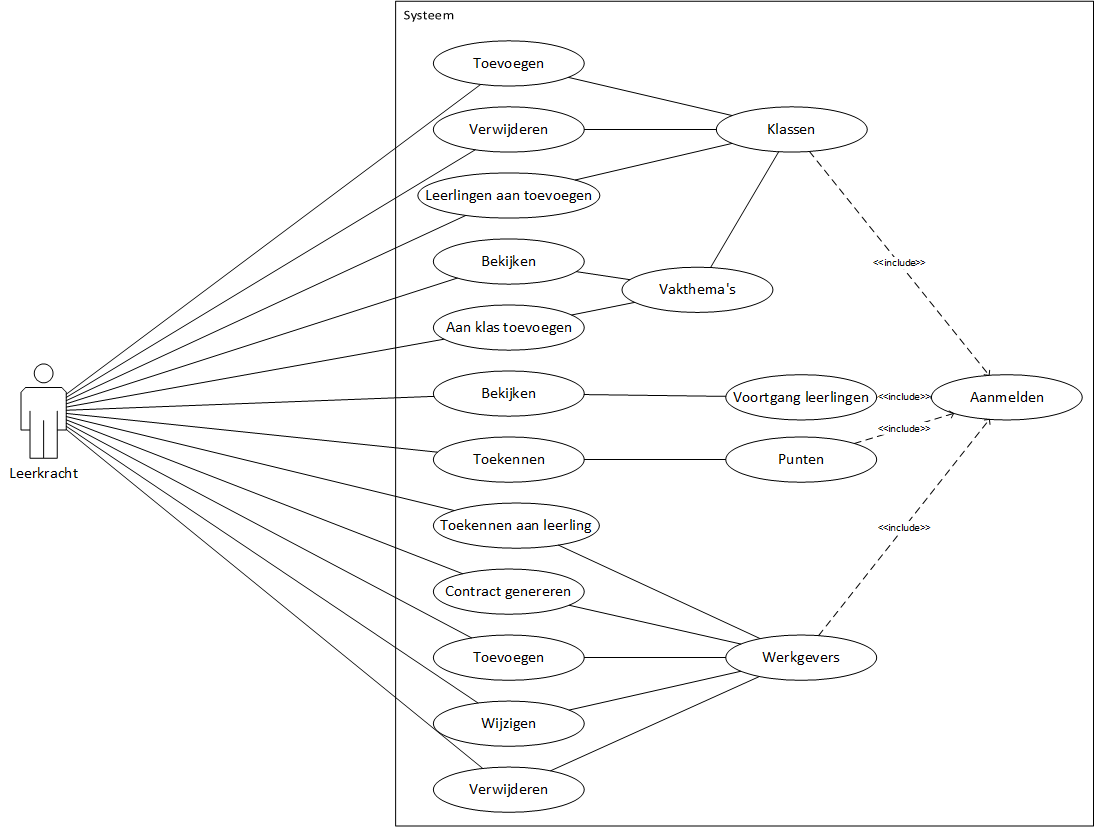
\includegraphics[width=\textwidth]{uc_leerkracht}
  \caption{Usecase diagram voor de leerkracht}
  \label{fig:usecase_leerkracht}
\end{figure}

%%%%%%%%%%%%%%%%%%%%%%%%%%%%%%%%%%%%%%%%%%%%%%%%%%%%%%%%%%%%%%%%%%%%%%%%%%%%%
%student
%%%%%%%%%%%%%%%%%%%%%%%%%%%%%%%%%%%%%%%%%%%%%%%%%%%%%%%%%%%%%%%%%%%%%%%%%%%%%
\todo{Use case commentaar Robin bespreken}
\newpage
\subsection{student}
% Voortgang bekijken
% !!!!!!!!!!! als je op een punt klikt krijg je een vakje met de commentaar te zien en voor pav het vakthema
% !!!!!!!!!!! toch nie mogelijk maken om in de voortgang punten aan te passen ? anders moet ge gaan kijken welke dag behaald en dan terug naar punten geven gaan wat veel stappen zijn
\begin{usecase}
    \addtitle{Use Case 11}{Voortgang bekijken} 
    \additemizedfield{Actoren}{
    	\item student
    }
    \addscenario{Beschrijving}{
        \item[] \textbf{Hoofdscenario:} \\
        Student meldt zich aan via de webapplicatie. Student kiest ``Voortgang''. De voortgang voor BGV en PAV staan in aparte tabs. Het systeem geeft een wekelijks overzicht van wanneer competenties(BGV)/doelstellingen(PAV) behaald werden door deze student.
    }
\end{usecase}

%Mobiele app - Tussentijd rapport
\begin{usecase}
    \addtitle{Use Case 12}{Mobiele app - Tussentijds rapport} 
    \additemizedfield{Actoren}{
    	\item student
    }
    \addscenario{Beschrijving}{
        \item[] \textbf{Hoofdscenario:} \\
        Student meldt zich aan via de mobiele applicatie. Student kiest ``Tussentijds rapport''. Het tussentijds rapport is opgedeeld in drie tabs nl. ``Alle'', ``BGV'' en ``PAV'' voor meer overzichtelijkheid. Het tussentijds rapport geeft een algemeen beeld van hoe de student het gedaan heeft tot nu toe a.d.v. cirkeldiagrammen (Per deelcertificaat/vakthema hoeveel competenties/doelstellingen ingeoefend en verworven zijn uit een totaal aantal te behalen competenties/doelstellingen).
    }
\end{usecase}

\todo{Invullen van scenario, takenstatus bekijken in de app.}
%Mobiele app - Tussentijd rapport
\begin{usecase}
    \addtitle{Use Case 13}{Mobiele app - Status taken} 
    \additemizedfield{Actoren}{
    	\item student
    	\item ouder
    }
    \addscenario{Beschrijving}{
        \item[] \textbf{Hoofdscenario:} \\
        Test
    }
\end{usecase}

\todo{usecase gaat over student, niet leerkracht}
\begin{figure}[H]
  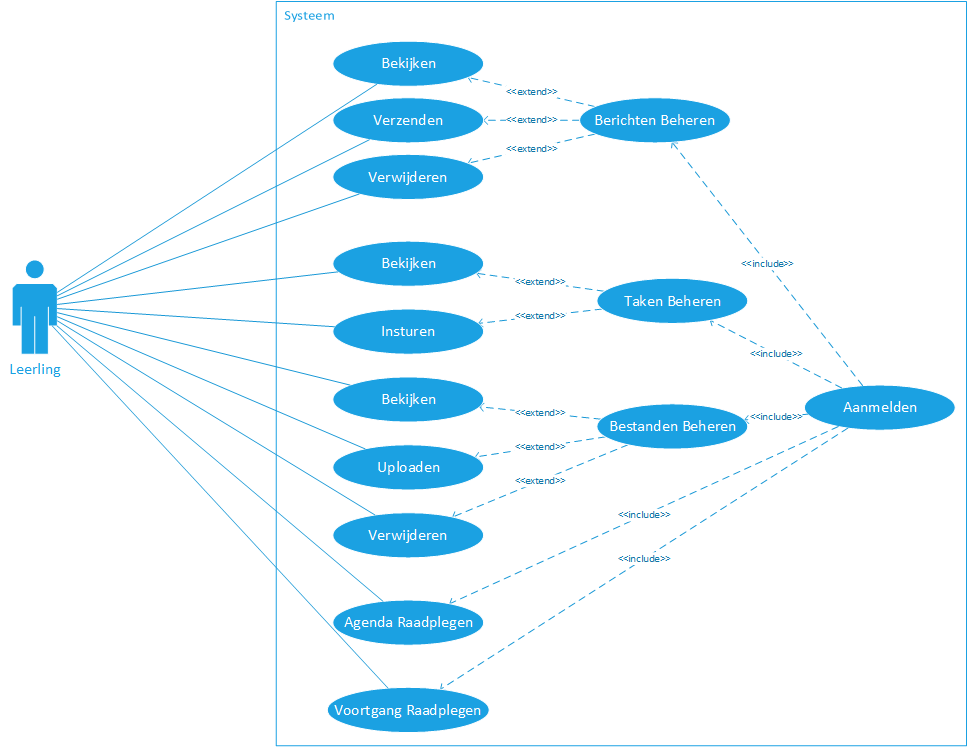
\includegraphics[width=\textwidth]{uc_leerling}
  \caption{Usecase diagram voor de student}
  \label{fig:usecase_student}
\end{figure}

%%%%%%%%%%%%%%%%%%%%%%%%%%%%%%%%%%%%%%%%%%%%%%%%%%%%%%%%%%%%%%%%%%%%%%%%%%%%%
%OUDER
%%%%%%%%%%%%%%%%%%%%%%%%%%%%%%%%%%%%%%%%%%%%%%%%%%%%%%%%%%%%%%%%%%%%%%%%%%%%%

\subsection{Ouder}

In alle use cases die in dit sectie voorkomen geldt de preconditie dat de ouder aangemeld is.

% Voortgang bekijken
\begin{usecase}
\addtitle{Use Case 14}{Voortgang bekijken} 
\additemizedfield{Actoren}{
	\item Ouder
}
\addscenario{Beschrijving}{
    \item[] \textbf{Hoofdscenario:} \\
    Ouder kiest kiest ``Voortgang''. De voortgang voor BGV en PAV staan in aparte tabs. Het systeem geeft een wekelijks overzicht van wanneer competenties(BGV)/doelstellingen(PAV) behaald zijn door het kind.\\
    \item[] \textbf{Alternatieve scenarios:} \\
    Indien de ouder meerdere kinderen heeft in de school, kan in een apart menu het gewenste kind geselecteerd worden.
}
\end{usecase}

%Mobiele app - Tussentijd rapport
\begin{usecase}
    \addtitle{Use Case 15}{Mobiele app - Tussentijds rapport} 
    \additemizedfield{Actoren}{
    	\item Ouder
    }
    \addscenario{Beschrijving}{
        \item[] \textbf{Hoofdscenario:} \\
        Ouder meldt zich aan via de mobiele applicatie. Ouder kiest ``Tussentijds rapport''. Het tussentijds rapport is opgedeeld in drie tabs nl. ``Alle'', ``BGV'' en ``PAV'' voor meer overzichtelijkheid. Het tussentijds rapport geeft een algemeen beeld van hoe dit kind het gedaan heeft tot nu toe a.d.v. cirkeldiagrammen (per deelcertificaat/vakthema hoeveel competenties/doelstellingen ingeoefend en verworven zijn uit een totaal aantal te behalen competenties/doelstellingen).\\
        \item[] \textbf{Alternatieve scenarios:} \\
        Indien de ouder meerdere kinderen heeft in de school, kan in een apart menu het gewenste kind geselecteerd worden.
    }
\end{usecase}

\begin{figure}[H]
  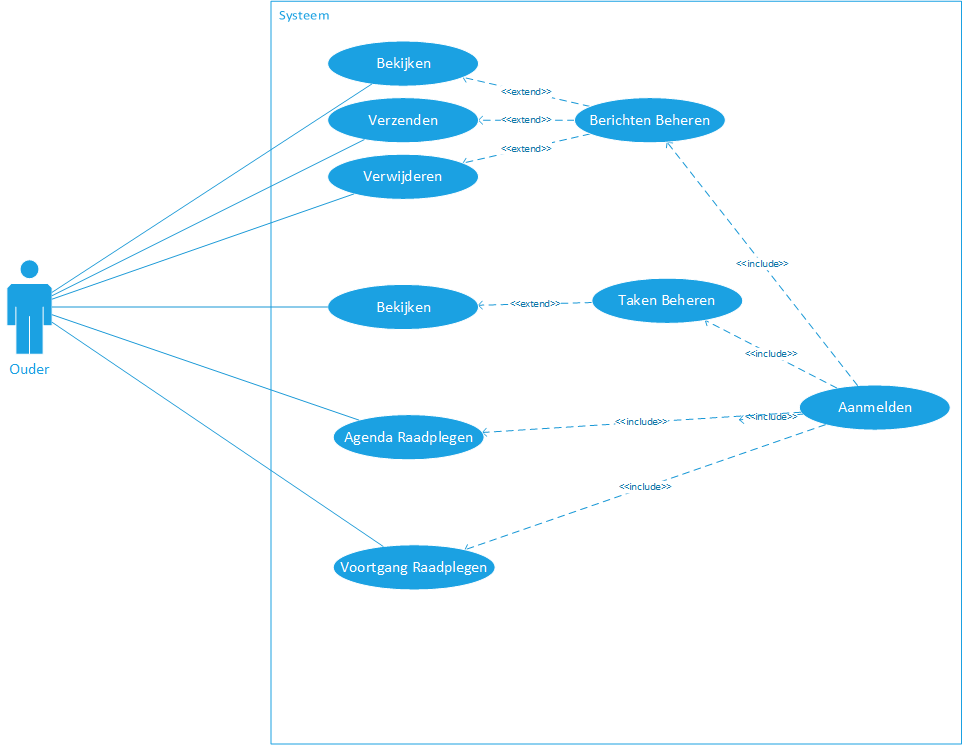
\includegraphics[width=\textwidth]{uc_ouder}
  \caption{Usecase diagram voor de ouder}
  \label{fig:usecase_ouder}
\end{figure}

% SSD's
\newpage
\section{Systeem sequentie diagrammen}
\subsection{Gebruiker toevoegen}
\begin{figure}[H]
  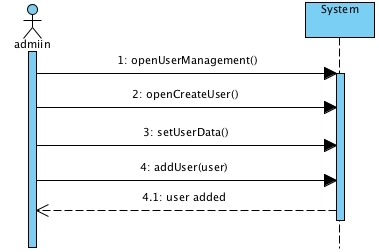
\includegraphics[width=\textwidth]{addUserSSD}
  \caption{Systeem sequentie diagram voor het toevoegen van een gebruiker}
  \label{fig:SSD_addUser}
\end{figure}

\subsection{Puntenbeheer}
\begin{figure}[H]
  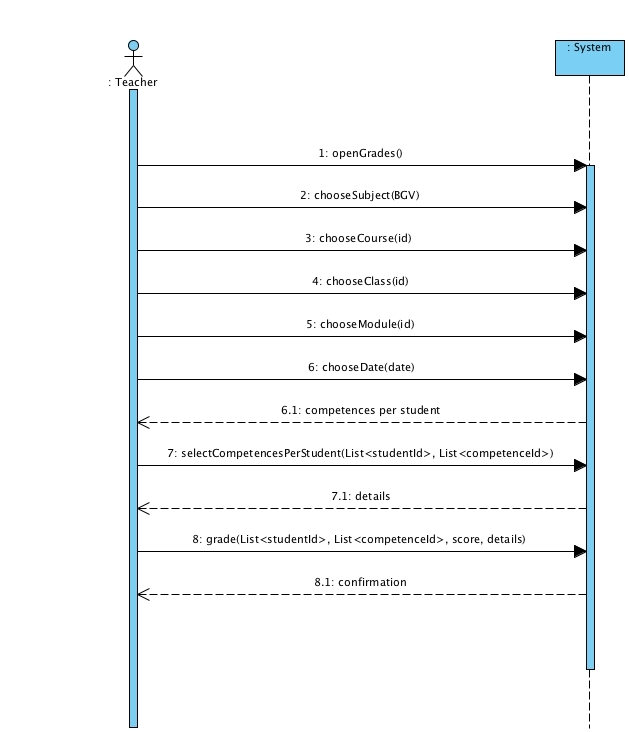
\includegraphics[width=\textwidth]{PuntenBeheerSSD}
  \caption{Systeem sequentie diagram voor het puntenbeheer}
  \label{fig:SSD_puntenbeheer}
\end{figure}

\newpage
\section{Contracten}
\subsection{Gebruiker toevoegen}
\begin{tabularx}{\textwidth}{|l X|}
    \hline
    \textbf{Naam} & openUserManagement() \\
    \textbf{Verwijzingen} & \begin{itemize}[leftmargin=*]
        \item Use Case 1 - Gebruiker toevoegen
        \item Systeem Sequentie Diagram 1 - Gebruiker toevoegen
    \end{itemize}\\
    \textbf{Pre-condities} & De beheerder is aangemeld.\\
    \textbf{Post-condities} & \begin{itemize}[leftmargin=*]
        \item Voor iedere bestaande gebruiker in de database wordt een kopie van het User object aangemaakt (om aan de front-end terug te geven); creatie van instantie.
    \end{itemize}\\
    \hline
\end{tabularx}\\

\begin{tabularx}{\textwidth}{|l X|}
    \hline
    \textbf{Naam} & openCreateUser() \\
    \textbf{Verwijzingen} & \begin{itemize}[leftmargin=*]
        \item Use Case 1 - Gebruiker toevoegen
        \item Systeem Sequentie Diagram 1 - Gebruiker toevoegen
    \end{itemize}\\
    \textbf{Pre-condities} & De beheerder is aangemeld.\\
    \textbf{Post-condities} & \begin{itemize}[leftmargin=*]
        \item Er wordt een nieuwe instantie van User aangemaakt; creatie van instantie.
    \end{itemize}\\
    \hline
\end{tabularx}

\begin{tabularx}{\textwidth}{|l X|}
    \hline
    \textbf{Naam} & setUserType(studentType) \\
    \textbf{Verwijzingen} & \begin{itemize}[leftmargin=*]
        \item Use Case 1 - Gebruiker toevoegen
        \item Systeem Sequentie Diagram 1 - Gebruiker toevoegen
    \end{itemize}\\
    \textbf{Pre-condities} & \begin{itemize}[leftmargin=*]
        \item De beheerder is aangemeld.
        \item Er bestaat een instantie van User, user genaamd.
    \end{itemize}\\
    \textbf{Post-condities} & \begin{itemize}[leftmargin=*]
        \item user.type werd studentType; aanpassing attribuut.
    \end{itemize}\\
    \hline
\end{tabularx}\\

\begin{tabularx}{\textwidth}{|l X|}
    \hline
    \textbf{Naam} & setInfo(userinfo) \\
    \textbf{Verwijzingen} & \begin{itemize}[leftmargin=*]
        \item Use Case 1 - Gebruiker toevoegen
        \item Systeem Sequentie Diagram 1 - Gebruiker toevoegen
    \end{itemize}\\
    \textbf{Pre-condities} & \begin{itemize}[leftmargin=*]
        \item De beheerder is aangemeld.
        \item Er bestaat een instantie van User, user genaamd, waarvoor user.type gekend is.
    \end{itemize}\\
    \textbf{Post-condities} & \begin{itemize}[leftmargin=*]
        \item user.naam werd userinfo.naam; aanpassing attribuut.
        \item user.voornaam werd userinfo.voornaam; aanpassing attribuut.
        \item \dots  (alle attributen die persoonlijke informatie voorstellen, staan in \ref{itm:student_info} opgesomd)
        \item user.username werd userinfo.username; aanpassing attribuut.
        \item user.password werd userinfo.password; aanpassing attribuut.
        \item user.email werd userinfo.email; aanpassing attribuut.
        \item user.pavklas werd userinfo.pavklas; aanpassing attribuut.
        \item user.bgvklas werd userinfo.bgvklas; aanpassing attribuut.
        \item user.inschrDatum werd userinfo.inschrDatum; aanpassing attribuut.
    \end{itemize}\\
    \hline
\end{tabularx}\\

\subsection{Puntenbeheer}
\begin{tabularx}{\textwidth}{|l X|}
    \hline
    \textbf{Naam} & openGrades() \\
    \textbf{Verwijzingen} & \begin{itemize}[leftmargin=*]
        \item Use Case 7 - Puntenbeheer
        \item Systeem Sequentie Diagram 2 - Puntenbeheer
    \end{itemize}\\
    \textbf{Pre-condities} & De leerkracht moet aangemeld zijn. De graden, certificaten, klassen en studenten moeten bestaan.\\
    \textbf{Post-condities} & \begin{itemize}[leftmargin=*]
        \item Het systeem houdt bij dat er punten geopend worden.
    \end{itemize}\\
    \hline
\end{tabularx}\\

\begin{tabularx}{\textwidth}{|l X|}
    \hline
    \textbf{Naam} & chooseSubject(BGV) \\
    \textbf{Verwijzingen} & \begin{itemize}[leftmargin=*]
        \item Use Case 7 - Puntenbeheer
        \item Systeem Sequentie Diagram 2 - Puntenbeheer
    \end{itemize}\\
    \textbf{Pre-condities} & De leerkracht moet aangemeld zijn. De graden, certificaten, klassen en studenten moeten bestaan.\\
    \textbf{Post-condities} & \begin{itemize}[leftmargin=*]
        \item Het systeem heeft het vak BGV ingeladen.
    \end{itemize}\\
    \hline
\end{tabularx}\\

\begin{tabularx}{\textwidth}{|l X|}
    \hline
    \textbf{Naam} & chooseCourse(id) \\
    \textbf{Verwijzingen} & \begin{itemize}[leftmargin=*]
        \item Use Case 7 - Puntenbeheer
        \item Systeem Sequentie Diagram 2 - Puntenbeheer
    \end{itemize}\\
    \textbf{Pre-condities} & De leerkracht moet aangemeld zijn. De graden, certificaten, klassen en studenten moeten bestaan. Het vak moet reeds geselecteerd zijn.\\
    \textbf{Post-condities} & \begin{itemize}[leftmargin=*]
        \item Het systeem heeft het vak met id ingeladen.
    \end{itemize}\\
    \hline
\end{tabularx}\\

\begin{tabularx}{\textwidth}{|l X|}
    \hline
    \textbf{Naam} & chooseClass(id) \\
    \textbf{Verwijzingen} & \begin{itemize}[leftmargin=*]
        \item Use Case 7 - Puntenbeheer
        \item Systeem Sequentie Diagram 2 - Puntenbeheer
    \end{itemize}\\
    \textbf{Pre-condities} & De leerkracht moet aangemeld zijn. De graden, certificaten, klassen en studenten moeten bestaan. Het vak moet reeds geselecteerd zijn.\\
    \textbf{Post-condities} & \begin{itemize}[leftmargin=*]
        \item Het systeem heeft de klas met id ingeladen.
    \end{itemize}\\
    \hline
\end{tabularx}\\

\begin{tabularx}{\textwidth}{|l X|}
    \hline
    \textbf{Naam} & chooseModule(id) \\
    \textbf{Verwijzingen} & \begin{itemize}[leftmargin=*]
        \item Use Case 7 - Puntenbeheer
        \item Systeem Sequentie Diagram 2 - Puntenbeheer
    \end{itemize}\\
    \textbf{Pre-condities} & De leerkracht moet aangemeld zijn. De graden, certificaten, klassen en studenten moeten bestaan. Het vak moet reeds geselecteerd zijn.\\
    \textbf{Post-condities} & \begin{itemize}[leftmargin=*]
        \item Het heeft de module met id ingeladen.
    \end{itemize}\\
    \hline
\end{tabularx}\\

\begin{tabularx}{\textwidth}{|l X|}
    \hline
    \textbf{Naam} & chooseDate(date) \\
    \textbf{Verwijzingen} & \begin{itemize}[leftmargin=*]
        \item Use Case 7 - Puntenbeheer
        \item Systeem Sequentie Diagram 2 - Puntenbeheer
    \end{itemize}\\
    \textbf{Pre-condities} & De leerkracht moet aangemeld zijn. De graden, certificaten, klassen en studenten moeten bestaan. Het vak moet reeds geselecteerd zijn.\\
    \textbf{Post-condities} & \begin{itemize}[leftmargin=*]
        \item Het systeem heeft de datum date ingesteld.
    \end{itemize}\\
    \hline
\end{tabularx}\\

\begin{tabularx}{\textwidth}{|l X|}
    \hline
    \textbf{Naam} & selectCompetencesPerStudent(List$<$studentId$>$, List$<$competenceId$>$) \\
    \textbf{Verwijzingen} & \begin{itemize}[leftmargin=*]
        \item Use Case 7 - Puntenbeheer
        \item Systeem Sequentie Diagram 2 - Puntenbeheer
    \end{itemize}\\
    \textbf{Pre-condities} & De leerkracht moet aangemeld zijn. De graden, certificaten, klassen en studenten moeten bestaan. Het vak moet reeds geselecteerd zijn.\\
    \textbf{Post-condities} & \begin{itemize}[leftmargin=*]
        \item Het systeem heeft de competenties met de studentId's en competenceId's ingeladen.
    \end{itemize}\\
    \hline
\end{tabularx}\\

\begin{tabularx}{\textwidth}{|l X|}
    \hline
    \textbf{Naam} & grade(List$<$studentId$>$, List$<$competenceId$>$, score, details) \\
    \textbf{Verwijzingen} & \begin{itemize}[leftmargin=*]
        \item Use Case 7 - Puntenbeheer
        \item Systeem Sequentie Diagram 2 - Puntenbeheer
    \end{itemize}\\
    \textbf{Pre-condities} & De leerkracht moet aangemeld zijn. De graden, certificaten, klassen en studenten moeten bestaan. Het vak moet reeds geselecteerd zijn.\\
    \textbf{Post-condities} & \begin{itemize}[leftmargin=*]
        \item Het systeem heeft de competenties met de studentId's en competenceId's score als score gegeven en feedback als details ingegeven.
    \end{itemize}\\
    \hline
\end{tabularx}\\



\clearpage
\section{Klassendiagram}
Omdat het onmogelijk is het volledige klassendiagram duidelijk te tonen, wordt het klassendiagram opgesplitst in verschillende delen die logisch samenhangen. In paragraaf \ref{uml_modellen} worden de modellen getoond zonder de objecten die nodig zijn voor de interactie met de database. De modellen zelf zijn opgesplitst in samenhangende delen. In paragraaf \ref{uml_voorbeeld} wordt voor \'e\'en model uitgewerkt hoe interactie met de database wordt gerealiseerd. Ook de bijhorende REST controller wordt getoond.

\subsection{Modellen} \label{uml_modellen}
\subsubsection{Accounts}
\begin{figure}[H]
  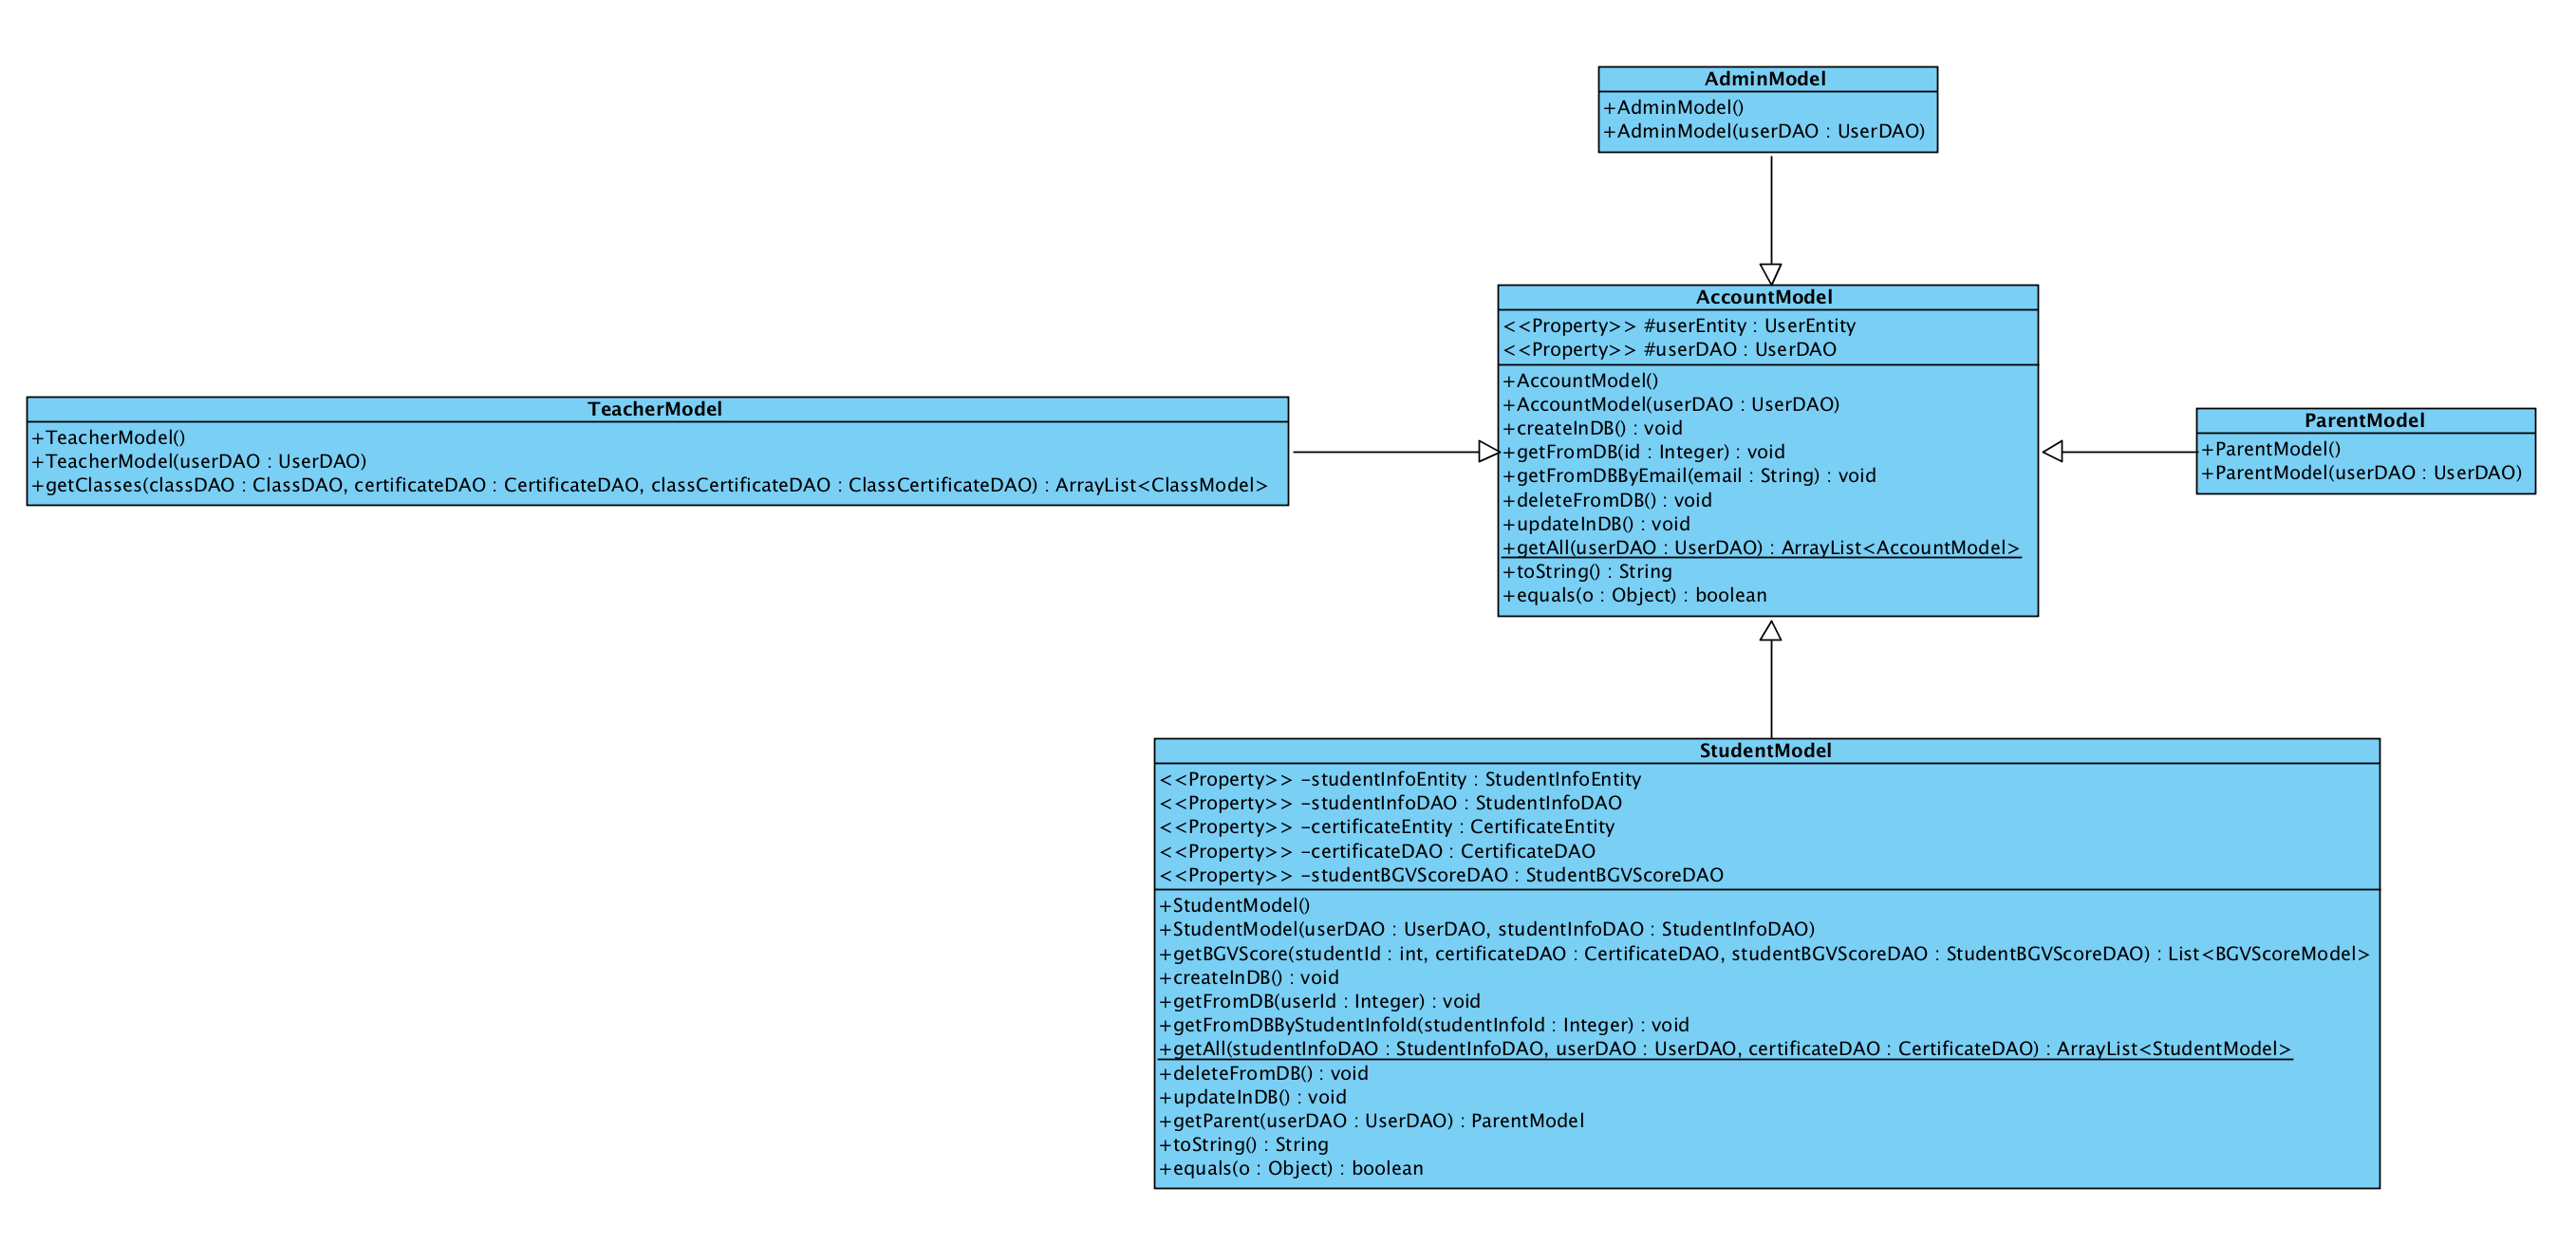
\includegraphics[width=\textwidth]{uml_accounts}
  \caption{Klassendiagram van accounts en afgeleiden.}
  \label{fig:uml_accounts}
\end{figure}

\subsubsection{Klassen}
\begin{figure}[H]
  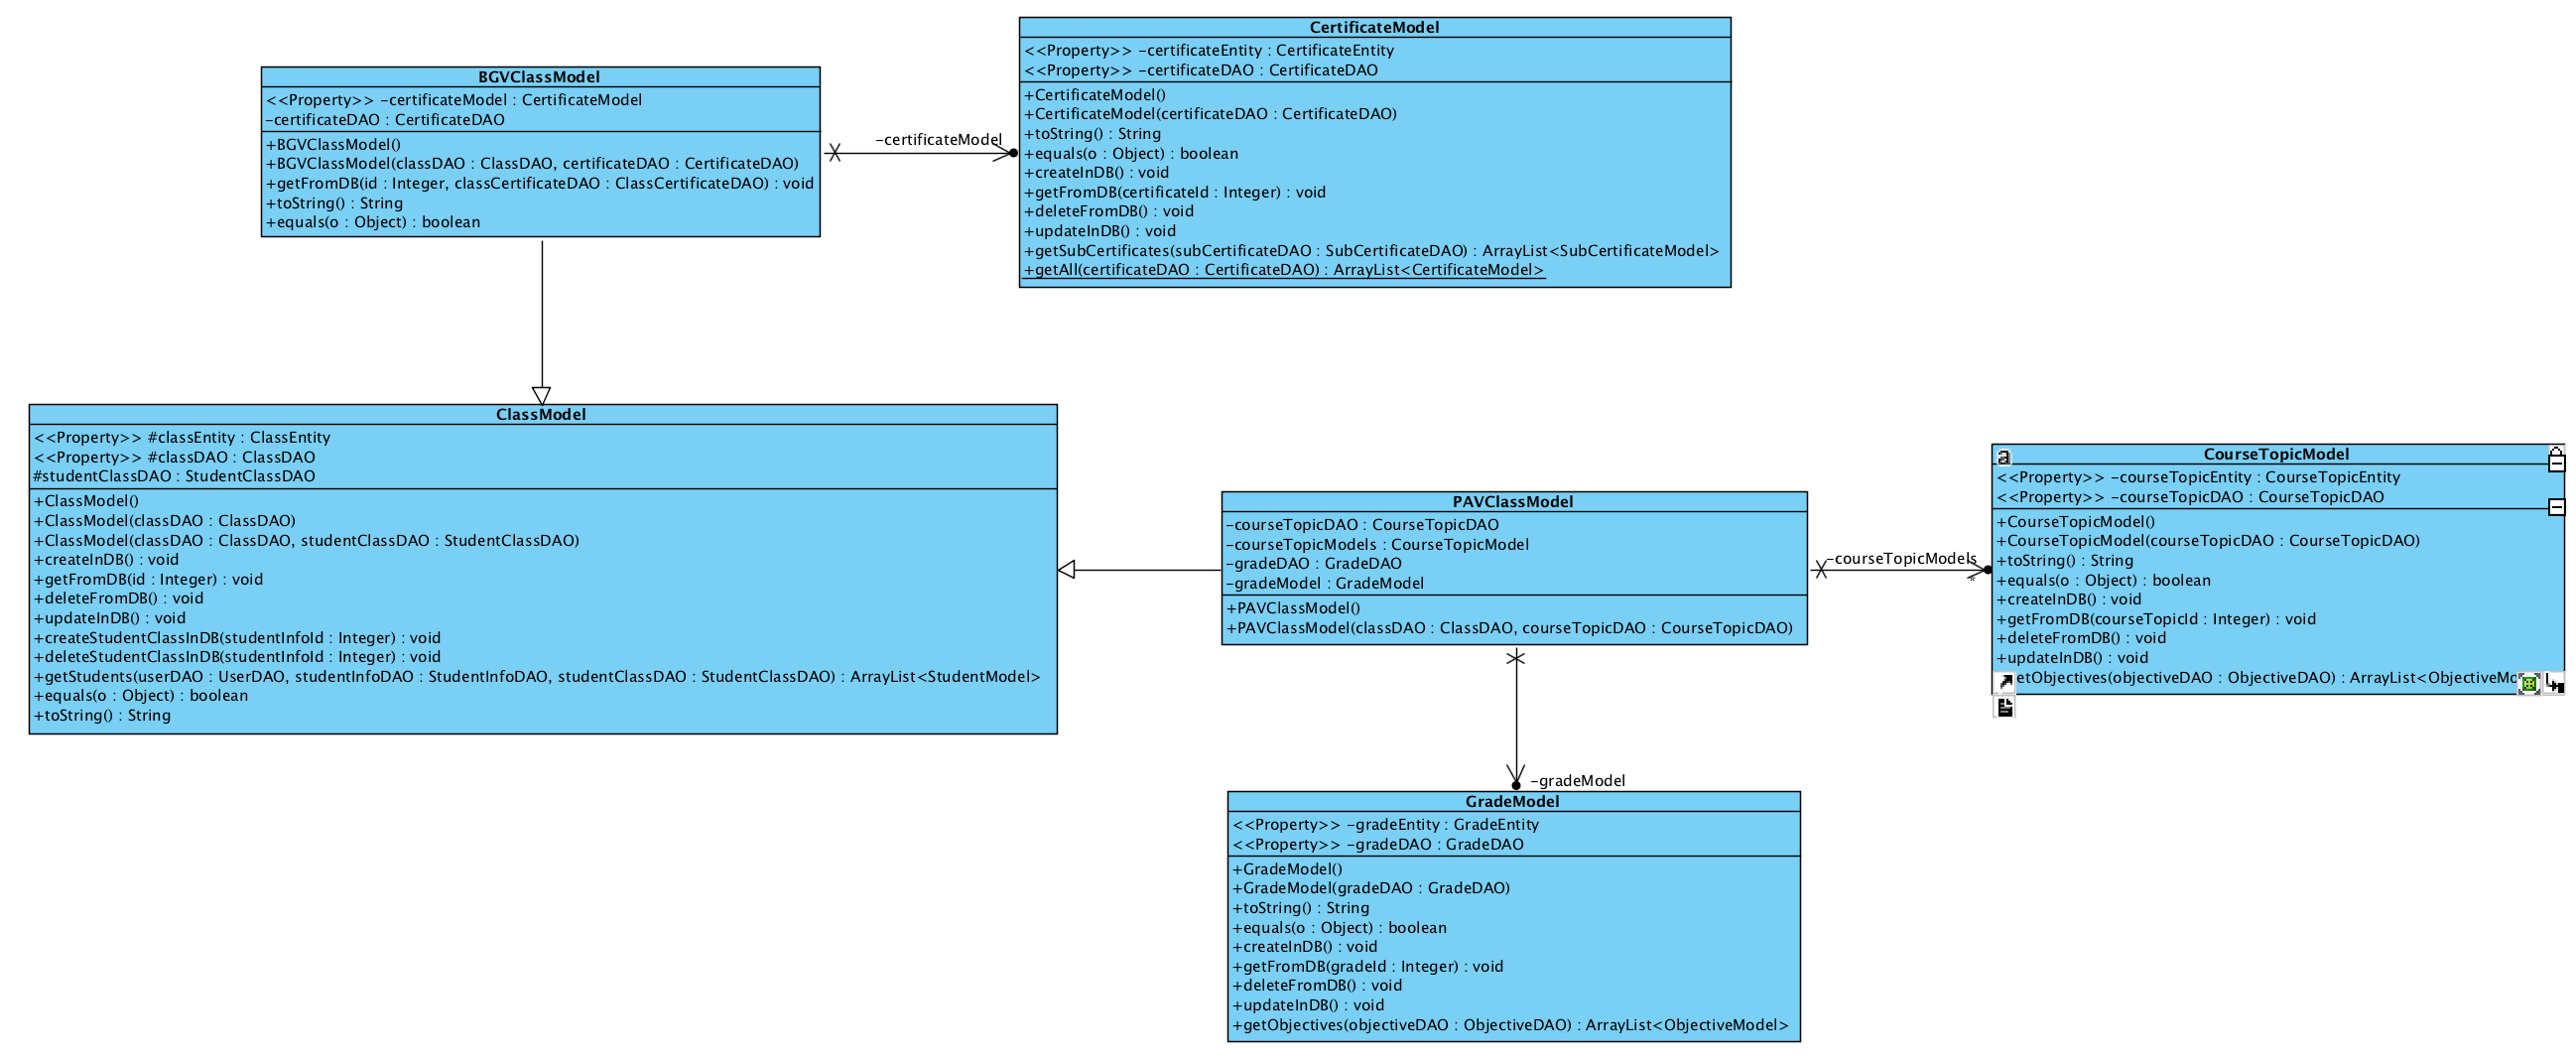
\includegraphics[width=\textwidth]{uml_klassen}
  \caption{Klassendiagram van klassen en alles errond.}
  \label{fig:uml_klassen}
\end{figure}


\subsubsection{Competenties, certificaten, scores}
\begin{figure}[H]
  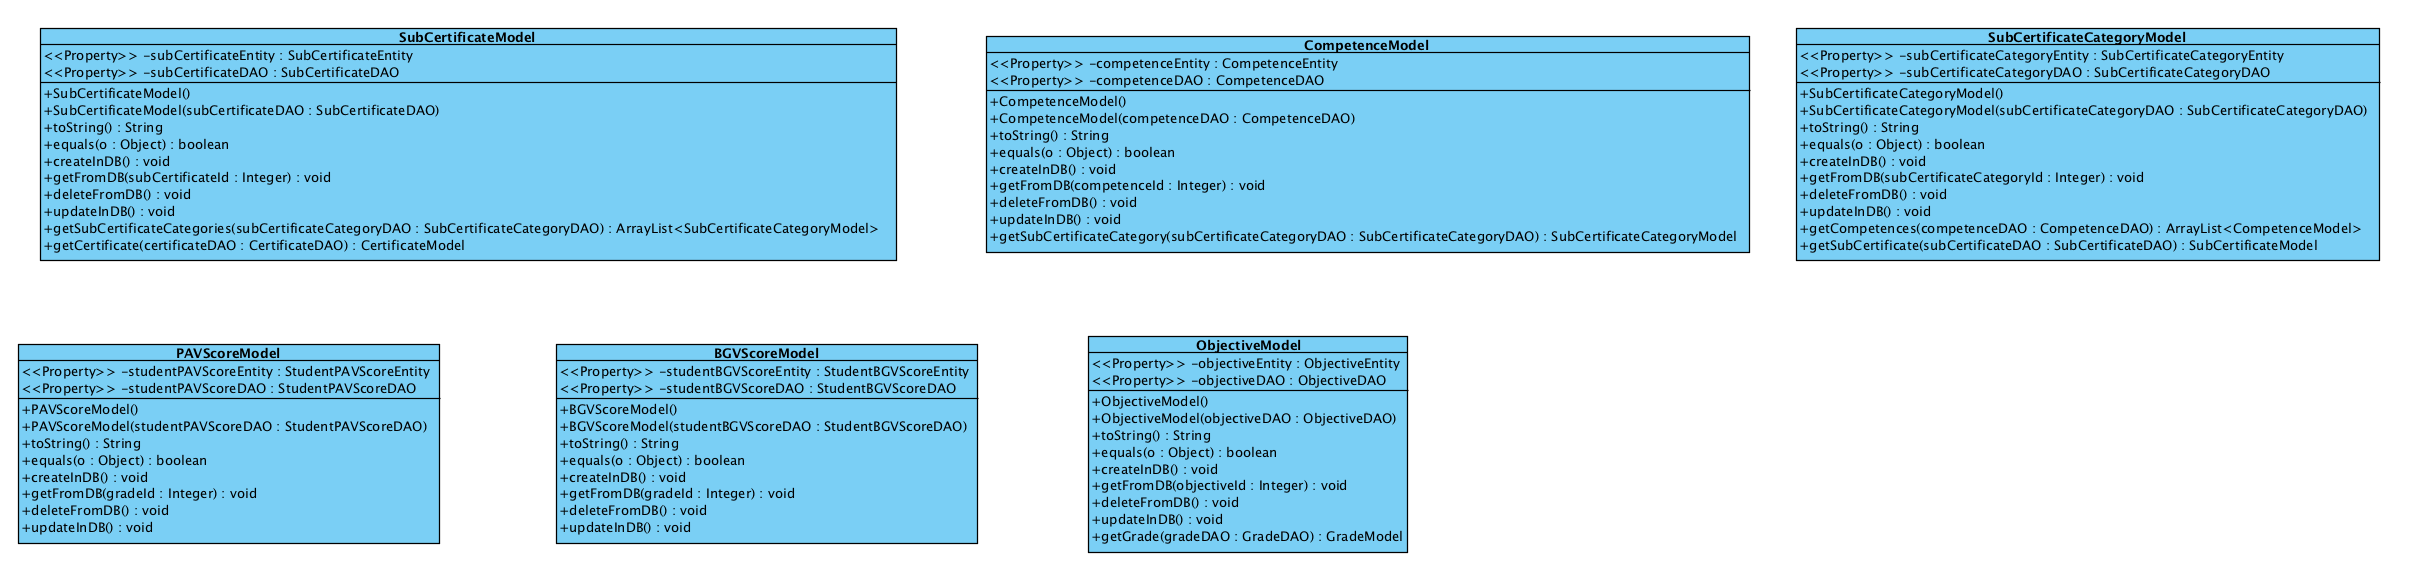
\includegraphics[width=\textwidth]{uml_rest}
  \caption{Klassendiagram van comptenties, certificaten en scores.}
  \label{fig:uml_rest}
\end{figure}

\subsection{Volledig uitgewerkt model} \label{uml_voorbeeld}
Om interactie met de database mogelijk te maken, voorzien we ten eerste een Entity (entiteit). Een entiteit is een 1 op 1 mapping met een tabel uit de database. Ten tweede gebruiken we een Data Acces Object (DAO) voor de interactie met de database. Deze implementeert typisch de CRUD-operaties (Create, Read, Update, Delete). Een DAO zelf maakt gebruik van de Java DataBase Connectivity (JDBC) API om SQL queries uit te voeren. Ten derde zorgt een RowMapper voor het invullen van een entiteit op basis van gequeryde data. Voor de modellen waarmee de web- en mobiele applicatie moeten kunnen interageren, wordt een REST controller voorzien. 

\begin{figure}[H]
  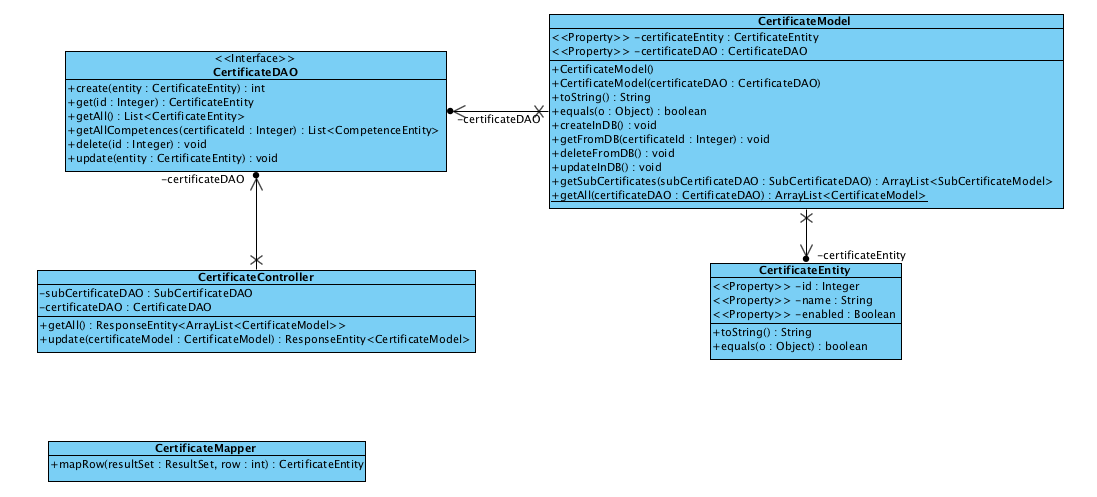
\includegraphics[width=\textwidth]{uml_voorbeeld}
  \caption{Voorbeeld waarbij niet enkel model getoond wordt.}
  \label{fig:uml_voorbeeld}
\end{figure}


\section{Entity-Relationship Diagram (ERD)}
Onderstaande figuur toont het ERD waarmee onze database opgesteld werd.
\begin{figure}[H]
  \centerline{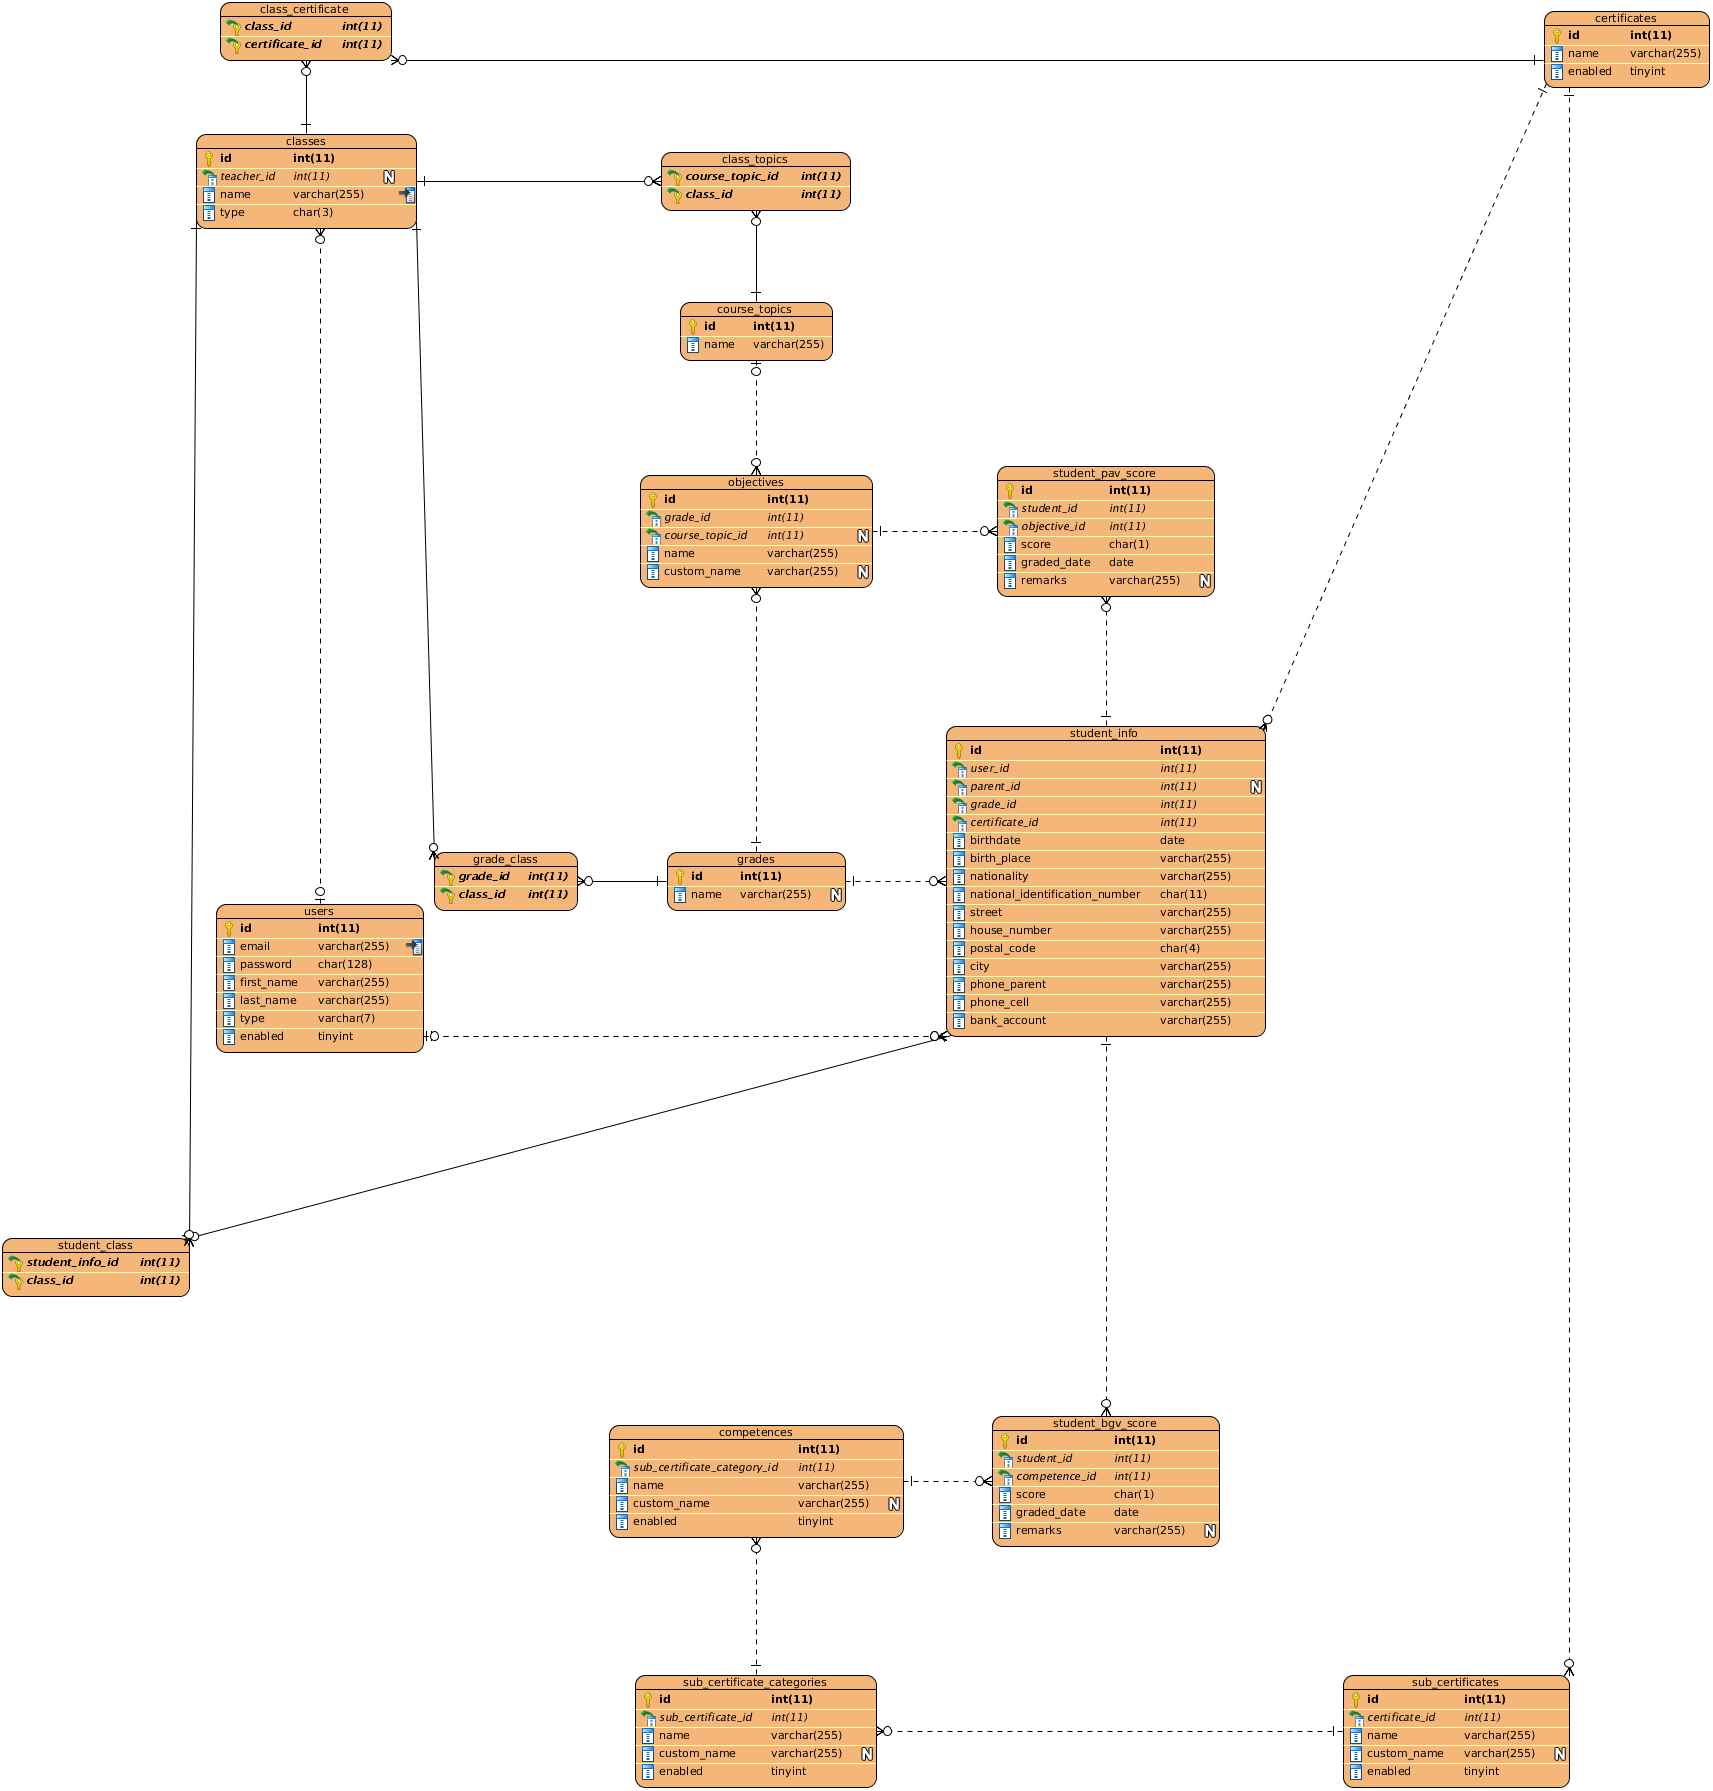
\includegraphics[width=\textwidth*4/5]{modulo}}
  \caption{ERD Schema}
  \label{fig:erd_schema}
\end{figure}




\newpage
\section{Scope}
\label{scope}
\subsection{Stap 1 (MVP)}
\begin{itemize} 
    \item Gebruikersbeheer
    \item Klassenbeheer
    \item Puntenbeheer
    \item Voortgang van studenten (web- en mobiele applicatie)
    \item Kunnen instellen of een certificaat door de school wordt aangeboden of niet.
\end{itemize}
Deze stap zien we als minimum viable product (MVP), en dus als scope voor het project van Software Engineering. 

\subsection{Stap 2}
\begin{itemize}
    \item Beheer van graden en certificaten
    \item Genereren van rapporten
\end{itemize}
Beide items in stap 2 zijn alleen front-end aanpassingen; de nodige support in de back-end moet in stap 1 reeds voorzien worden. Het zou dus niet zo veel tijd kosten om te voorzien, maar aangezien dit voor de opdrachtgever niet zo belangrijke functionaliteiten zijn, voorzien we ze pas in stap 2.

\subsection{Stap 3}
\begin{itemize}
    \item Werkgeversbeheer
    \item Genereren van werkgeverscontracten
\end{itemize}



\section{Methodologie}
Er wordt per 2 aan eenzelfde module gewerkt. In het begin maken we gebruik van pair programming, om Spring en AngularJS beter te leren kennen. We hebben hier nog geen ervaring mee. Daarna zullen we met 2 aan eenzelfde module werken, zodat de teamleden elkaar snel verder kunnen helpen in geval van moeilijkheden. Ook wisselen de teams regelmatig van module, zodat alle leden van het ontwikkelingsteam minstens een basiskennis hebben van alle code (front-end, back-end en Android).



\newpage
\section{Planning}
\subsection{Analyse}
\begin{enumerate}
    \item \textbf{29/03:}\\
    Analyse: feedback van klant over analyseverslag werwerken in verslag.\\
    Het hele team werkt hier samen aan.
    \item \textbf{03/04 en 04/04:}\\
    Analyse: feedback van onderwijsteam verwerken in verslag.\\
    Het hele team werkt hier samen aan.
\end{enumerate}


\subsection{Eerste iteratie}
Eerst geven we de planning opgesteld vóór de eerste iteratie van start ging. We voorzien $4$ werkdagen per week. Vervolgens wordt besproken hoe we er van zijn afgeweken.
\begin{enumerate}[resume]
    \item \textbf{05/04:}\\
    Design: high-level UML, interactiediagrammen, en databasemodel.\\
    Installeren van alle IDE's en SDK's.\\
    Het hele team werkt hier samen aan.
    \item \textbf{06/04:}\\
    Opzetten van een basisproject voor de back-end, front-end en Android-app. Basisproject bevat interactie met database, als test.\\
    Het hele team werkt hier samen aan.
    \item \textbf{07 en 08/04:}\\
    Front-end: Vertrouwd raken met AngularJS en Bootstrap. Opbouwen van Single Page App en algemene structuur van het project. Reinaert en Jens.\\
    Back-end: Vertrouwd raken met Spring. Alle entiteiten en DAO's voorzien, met bijhorende unit-tests. Martijn, Hendrik, Vincent en Michiel.
    \item \textbf{11 en 12/04:}\\
    Front-end: Backend simulatie implementeren. Reinaert, Jens en Martijn.\\
    Back-end: Alle Model's implementeren. Vincent en Michiel.\\
    Android: Layout om voortgang te tonen met dummy data. Hendrik.
    \item \textbf{14, 15 en 18/04:}\\
    Front-end: Gebruikersbeheer, Michiel en Vincent. Login systeem, Hendrik.\\
    Back-end: Een aantal test Controller's aanmaken en de controller voor gebruikerbeheer. Reinaert, Martijn en Jens.\\
    Certificate crawler: Automatisch certificaten inladen, Reinaert.
    \item \textbf{20, 21 en 22/04:}\\
    Front-end: Voorzien van selecteerbaar matrix voor puntenbeheer, Reinaert en Jens. Voorzien van overige fucntionaliteiten voor puntenbeheer, Michiel en Vincent.\\
    Back-end: Controller(s) voorzien voor puntenbeheer, Hendrik en Martijn.\\
\end{enumerate}

In het begin hebben we ons aan bovenstaande planning kunnen houden. De bedoeling was om zo snel mogelijk met de belangrijkste en meest complexe module, puntenbeheer, te beginnen. Maar het vertrouwd raken met AngularJS, Bootstrap en Spring was moeilijker dan verwacht. Daarom zijn we begonnen met het realiseren van de eenvoudigere componenten en lag de focus in het begin vooral op de back-end. Momenteel, aan het einde van de eerste iteratie dus, hebben we het onderstaande gerealiseerd. De namen die bij ieder puntje vermeld worden, zijn de personen die hier het grootste deel van gerealiseerd hebben.

\begin{itemize}
    \item Login:\\
    Er wordt gecheckt of de combinatie username-password geldig is. Front-end door Reinaert en back-end door Vincent. Gebruik van een token moet nog gebeuren.
    
    \item Gebruikersbeheer:\\
    Lijst van gebruikers wordt opgevraagd uit database. Paginering is niet klaar. Mogelijkheid om gebruikers te zoeken wel, door Vincent. Aanmaken en bewerken van een gebruiker is mogelijk, behalve het instellen van de graad en het certificaat. Instellen of een gebruiker (in)actief is, is ook klaar. instellen (in)actief en melding voor gebruikers te verwijderen door Jens. Front-end door Michiel en Reinaert. Back-end door Vincent. 
    
    \item Klassenbeheer:\\
    De lijst van PAV klassen is alleen aan front-end klaar; niet in back-end. De BGV klassen worden wel uit database opgehaald, en is dus ook klaar in back-end. Een BGV klas kan verwijderd worden. Het aanmaken van een klas is klaar, maar nog zonder koppeling tussen front- en back-end. Het verwijderen van een student uit een klas is wel gekoppeld. Het aanmaken van vakthema's is af, maar nog zonder koppeling tussen front- en back-end. Back-end door Vincent. Front-end door Jens, lijst en tree-view studenten door Martijn (inclusief back-end aanvulling voor de nodige functionaliteiten en koppeling). 
    
    \item Puntenbeheer:\\
    Voor de back-end is dit helemaal klaar. Voor de front-end kunnen nog geen scores geselecteerd worden in het matrix, maar de rest is wel volledig klaar. Er is ook nog geen koppeling met de back-end. Back-end door Michiel. Front-end door Jens en Reinaert. 
    
    \item Voortgang van studenten:\\
    Nog niets klaar aan front-end. Back-end hiervoor is die van puntenbeheer.
    
    \item Certificaten:\\
    Men kan instellen of een certificaat al dan niet wordt aangeboden. Nog geen zoekfunctionaliteit. Back-end (inclusief subcertificaten en competenties) door Michiel. Front-end door Martijn.
    
    \item Android:\\
    UI om scores te tonen is klaar, maar gebruikt nog dummy data. De naam waarmee men zogezegd is aangemeld, wordt uit de database opgehaald. Door Hendrik.
    
    \newpage
    \item Certificate crawler:\\
    Een Python script is geschreven om automatisch certificaten en deelcertificaten af te halen van de website van de Vlaamse overheid en deze om te zetten in SQL queries zodat ze in de back-end opgeslagen kunnen worden, door Reinaert.
\end{itemize}

Ondanks we bepaalde onderdelen uit de planning voor de eerste iteratie niet hebben gerealiseerd, hebben we wel reeds delen gerealiseerd die oorspronkelijk voor de tweede iteratie gepland waren. In het algemeen staat de back-end nu dus verder dan gepland, maar de front-end iets minder ver.


\subsection{Tweede iteratie}
In de tweede iteratie voorzien we $3$ werkdagen per week.
\begin{enumerate}[resume]
    \item \textbf{25 t.e.m.\ 29/04:}\\
    In deze periode voorzien we \'e\'en dag voor feedback van klant; nog niet geweten welke precieze datum. De overige twee dagen voorzien we voor allerlei kleine aanpassingen aan de database, front- en back-end. De bedoeling is ook enkele eenvoudige koppelingen (tussen front- en back-end) te realiseren. Het hele team werkt hier aan.
    
    \item \textbf{02 t.e.m.\ 06/05:}\\
    Graad en opleiding kunnen instellen bij gebruikersbeheer, door Michiel. Gebruik van een authentication token bij login, en het parsen van competenties in de certificate crawler, door Reinaert. Voorzien van zoekfunctionaliteit in certificaten, door Vincent. Voortgang van studenten tonen in webapplicatie, door Hendrik en Martijn. Koppeling van vakthema's, door Jens.
    
    \item \textbf{09 t.e.m.\ 13/05:}\\
    Het selecteerbaar maken van de matrix voor puntenbeheer, door Reinaert. Koppeling (tussen front- en back-end) voor puntenbeheer, door Jens. Het voorzien van een PAV klas in de back-end en bijhorende koppeling in de front-end, door Hendrik. Wisselen van tabs in Android app, door Martijn. Login systeem voor Android applicatie, door Vincent. Keuze van te beschouwen kind in Android app en koppeling met back-end, door Michiel.
    
    \item \textbf{16 t.e.m.\ 20/05:}\\
    Deze dagen worden voorzien voor bug-fixes, last-minute aanpassingen en het updaten van het verslag. Het hele team werkt hier aan.
\end{enumerate}



\newpage
\section{Systeem evolutie}
Onderstaande modules zijn mogelijke uitbreidingen, na de $3$ stappen uit de scope (zie \ref{scope}). Ze staan geordend op prioriteit.
\begin{enumerate}
    \item Interne agenda waarin systeembeheerders lessen en algemene activiteiten kunnen inplannen. Extra functionaliteiten hierbinnen zijn de mogelijkheid om naar iCal te exporteren en meldingen te ontvangen in geval van last-minute wijzigingen.
    \item Een intern berichtensysteem waarmee gebruikers met elkaar kunnen communiceren. Hierin zouden de typische functionaliteiten zitten, zoals een bericht versturen, verwijderen, doorsturen, bijlages toevoegen.
    \item Een bestandsbeheersysteem waarin een gebruiker bestanden kan uploaden, en deze beheren (hernoemen, verwijderen, downloaden).
    \item Een takensysteem waarin leerkrachten een taak kunnen opleggen voor een bepaald vakthema. De studenten hebben de mogelijkheid om een bestand (= de taak) te uploaden.
\end{enumerate}


\newpage
\begin{appendices}
\section{Mockups webapplicatie}

\begin{figure}[H]
  \centerline{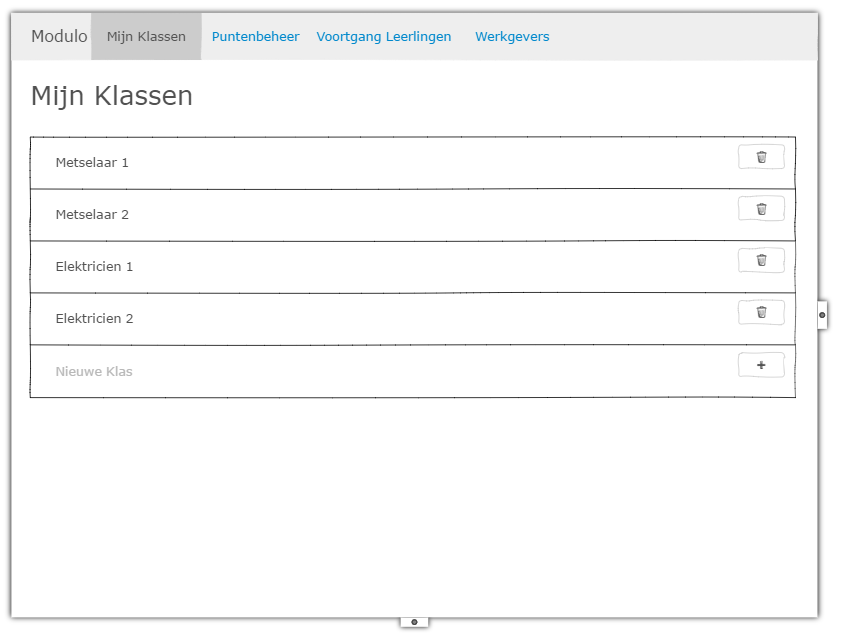
\includegraphics[width=\textwidth]{web_klassen}}
  \caption{Lijst van klassen van een leerkracht}
  \label{fig:web_klassen}
\end{figure}

\begin{figure}[H]
  \centerline{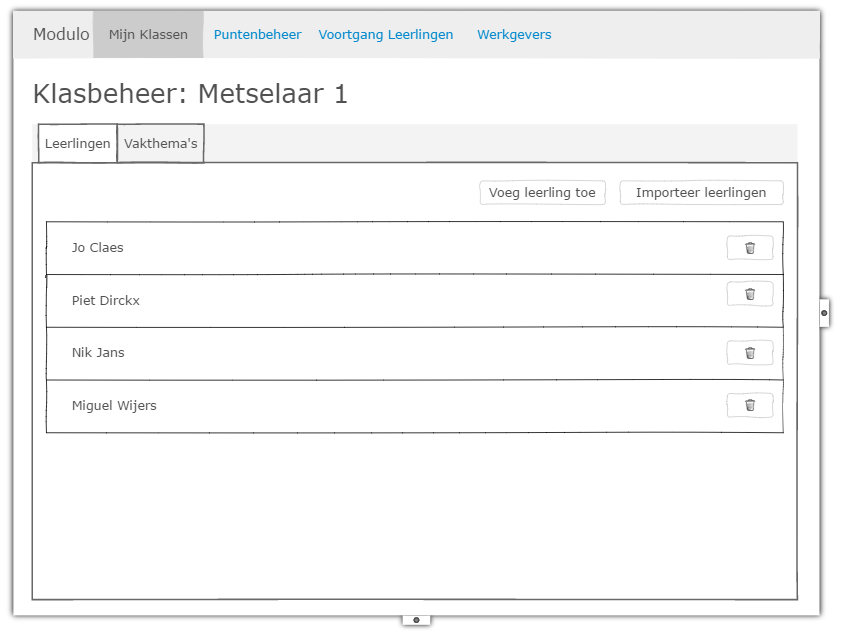
\includegraphics[width=\textwidth]{web_klasbeheer}}
  \caption{Beheer van een klas}
  \label{fig:web_klasbeheer}
\end{figure}

\begin{figure}[H]
  \centerline{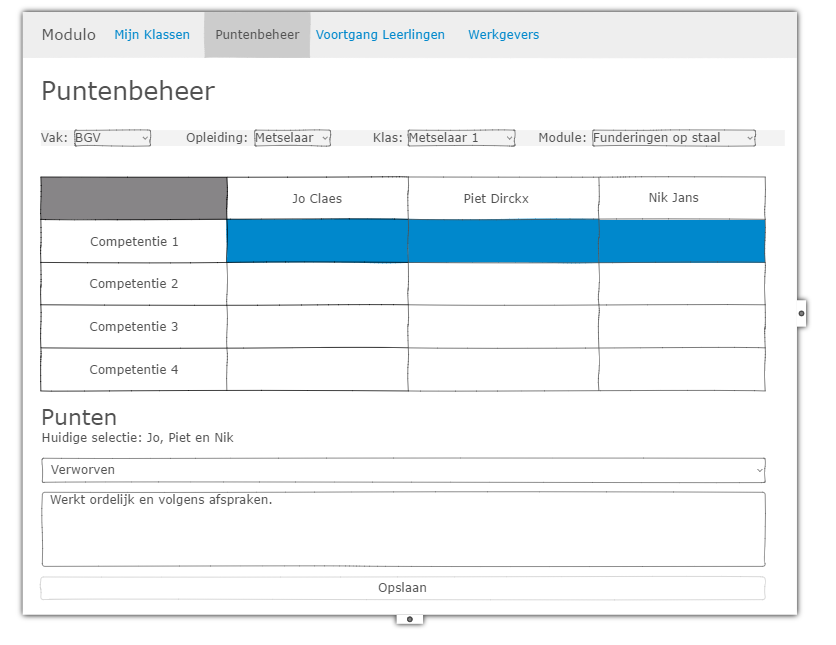
\includegraphics[width=\textwidth]{web_punten}}
  \caption{Opzoeken en toekennen van punten}
  \label{fig:web_punten}
\end{figure}

\begin{figure}[H]
  \centerline{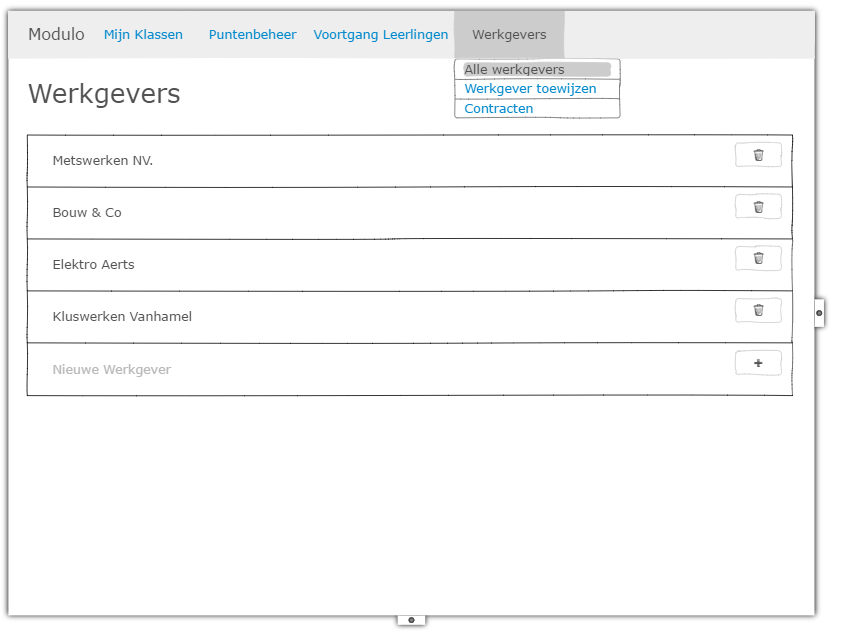
\includegraphics[width=\textwidth]{web_werkgevers_dropdown}}
  \caption{Dropdown werkgevers}
  \label{fig:web_werkgevers_dropdown}
\end{figure}
\newpage


\newpage
\section{Mockups mobiele applicatie}

% \begin{figure}[H]
%   \centerline{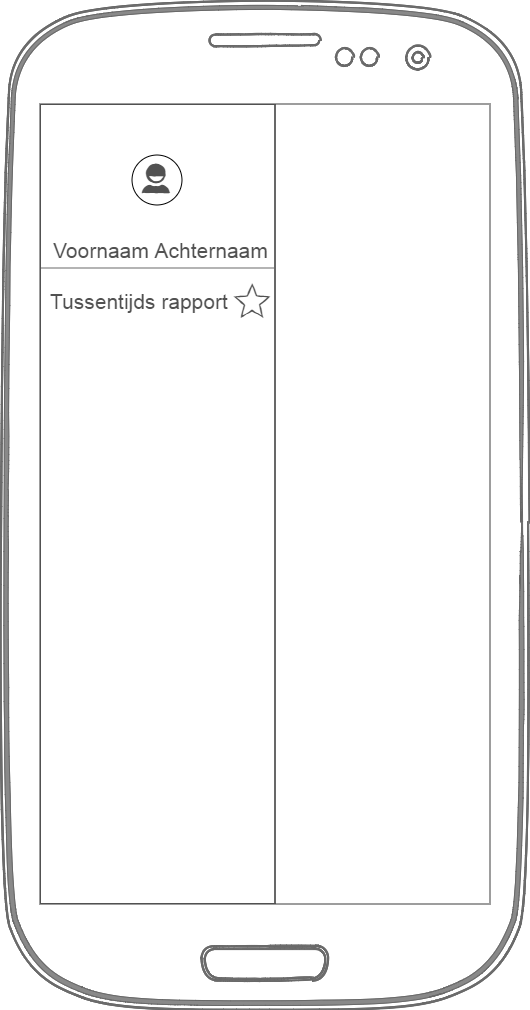
\includegraphics[width=\textwidth*4/5]{MobieleApp/leerling_view}}
%   \caption{Menu voor studenten}
%   \label{fig:mobiel_student}
% \end{figure}

% \newpage
% \begin{figure}[H]
%   \centerline{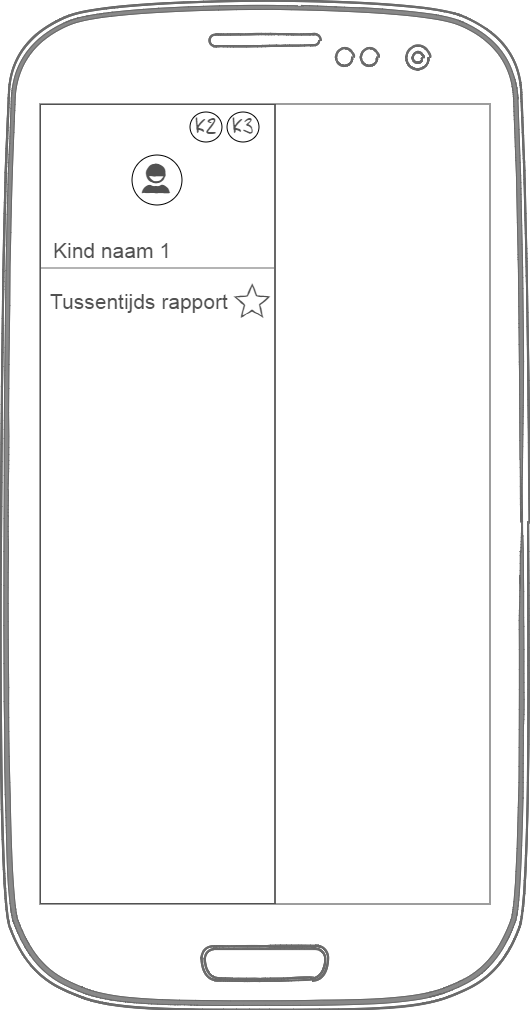
\includegraphics[width=\textwidth*4/5]{MobieleApp/ouders_view}}
%   \caption{Menu voor ouders}
%   \label{fig:mobiel_ouder}
% \end{figure}

% \newpage
\begin{figure}[H]
  \centerline{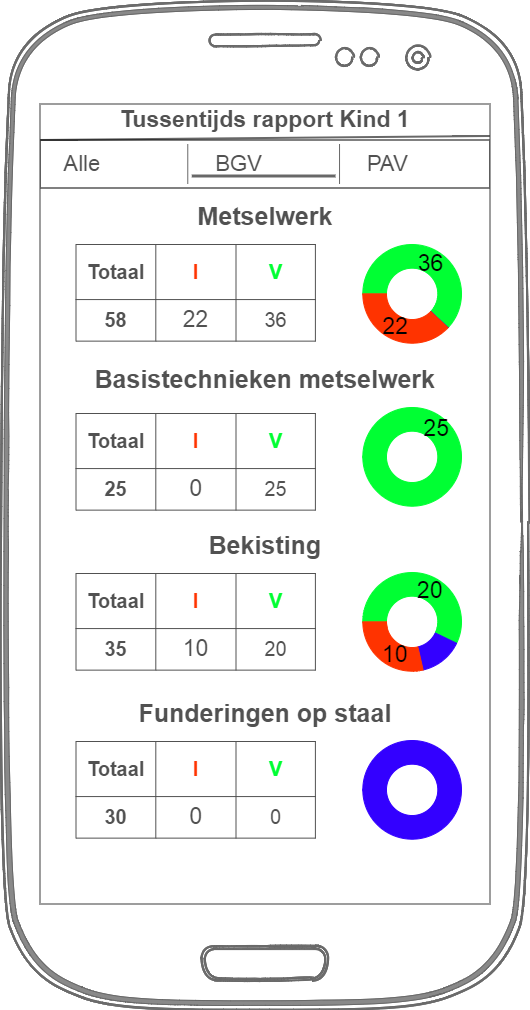
\includegraphics[width=\textwidth*4/5]{MobieleApp/tussentijds_rapport}}
  \caption{Tussentijds rapport}
  \label{fig:mobiel_tussentijds_rapport}
\end{figure}


\newpage
\includepdf[pages={1},scale=0.75,pagecommand=\section{Voorbeeld van een contract}\label{vbContract}]{vbcontract.pdf}
\includepdf[pages=2-,scale=0.75,pagecommand={}]{vbcontract.pdf}


\end{appendices}

\newpage
\bibliography{Referenties}
\bibliographystyle{unsrt}

\end{document}

%  Gebruikersbeheer
%  Mijn klassen
%       Lijst van klassen (en toevoegen, verwijderen klassen))
%           klasbeheermenu (studenten toevoegen/verwijderen, vakthema's toevoegen (met tellertjes per doelstelling die aangeven hoeveel keer een doelstelling reeds in de vakthema's zit), optie bij vakthema toevoegen om er een remediëringstaak van te maken en geeft lijst van studenten, vakthema's verwijderen)
%
%  Puntenbeheer
%       bgv / pav
%           certificaat / graad
%               klas / klas
%                   bgv -> deelcertificaat / pav -> vakthema
%
%  Voortgang studenten
%       voortgang per student
%       rapporten afdrukken
%
%  Werkgeversbeheer
%       contracten
%       werkgevers
%       werkgever toewijzen
%
%  graden/certificaten (competenties/doelstellingen)
%       om te bewerken kiezen welk vak, dan graad/opleding, deelcertificaat en dan wijzigen 

% indien we een doelstelling of competentie 3keer verworven hebben dan gaan we alle dagen uitgrijzen behalve de dage waarop de doelstelling verworven is zodat we deze nog kunnen aanpassen


% vier tabs: vier verschillende gebruikers, een niet ingelogd, rest wel
% toon leerling: hier komt puntending, nog niet af
% ouder: hetzelfde
% leerkracht: toon lijsten van klassen, klik klas toevoegen, leg uit hoe het werkt, klas bewerken, dan puntenbeheer
%


%%%% Draaiboek
% Website:
% 	leerling
% 		aanmelden
% 		vertellen wat hier komt, wat leerling kan
% 		enkel frontend
% 		afmelden

% 	ouder
% 		al aangemeld
% 		vertellen wat hier komt, wat ouder kan
% 		enkel frontend

% 	leerkracht
% 		mijn klassen
% 			PAV lijst van klassen, enkel frontend
% 			BGV
% 				lijst van klassen
% 				klas toevoegen -> leerlingen db data, enkel frontend bruikbaar
% 				klas bewerken
% 					leerlingen toevoegen -> volledig backend
% 					leerlingen verwijderen -> volledig backend
% 				vakthema's -> dummy data, frontend
% 					bewerken
% 					toevoegen
% 				details
% 					klasnaam -> frontend
% 		puntenbeheer -> volledig frontend, dummy data
% 			gewoon even uitleggen en bespreken
% 		voortgang leerlingen
% 		 	uitleggen wat er komt


% 	beheerder
% 		gebruikersbeheer -> volledig backend, maar niet volledig af
% 			lijst van users uit backend/db
% 			zoeken op user
% 			nieuwe gebruiker aanmaken (standaarddata) -> werkt nog niet
% 			gebruiker bewerken (gelijkenis nieuwe) 
% 				ouder koppelen
% 			verwijderen (uit backend)
% 			paginering werkt nog niet
% 		certificaten
% 			lijst die enabled/disabled kan worden -> komen uit backend
% 			hier komt ook zoekfunctionaliteit zoals gebruikersbeheer (2e iteratie)

% Android
% 	naam waarmee ingelogd is komt uit backend/db
% 	UI met dummy data
% 	inlogscherm moet nog komen
% 	tabs tussen PAV,BGV, algemeen
%  	kind kiezen